\chapter{STDP Training on Spiking Deep Learning Models}
\label{cha:sdlm}
%Paragraph One: LINK
%Make a connection to what has immediately gone before. Recap the last chapter. In the last chapter I showed that… Having argued in the previous chapter that… As a result of x, which I established in the last chapter….. It is also possible to make a link between this chapter and the whole argument… The first step in answering my research question (repeat question) .. was to.. . In the last chapter I …
Having argued in the previous chapter that it is feasible to construct deep SNNs off-line by training DNN with specific activation function.
This Chapter continues the hot topic of deep SNNs and takes extra step forward to on-line, spike-based training in biologically plausible manner.

%Paragraph Two: FOCUS
%Now focus the reader’s attention on what this chapter is specifically going to do and why it is important. In this chapter I will examine.. I will present… I will report … This is crucial in (aim of thesis/research question) in order to….
In this Chapter We will present the approach which successfully transfers the discrete weights update of conventional unsupervised training of deep learning modules to spike-based STDP learning.
It is crucial in not only building SNNs for object recognition applications, but also equipping the deep SNN models with biologically plausible learning capability.
It is also attractive and promising to implement the on-line, event-based training algorithm on neuromorphic hardware for better power efficiency and scalability.


%Paragraph Three: OVERVIEW
%The third paragraph simply outlines the way that you are going to achieve the aim spelled out in the previous paragraph. It’s really just a statement of the contents in the order that the reader will encounter them. It is important to state these not simply as topics, but actually how they build up the internal chapter argument… I will begin by examining the definitions of, then move to seeing how these were applied… I first of all explain my orientation to the research process, positioning myself as a critical scholar.. I then explain the methodology that I used in the research, arguing that ethnography was the most suitable approach to provide answers to the question of… 
%https://patthomson.net/2014/01/16/connecting-chapterschapter-introductions/
We first of all explore the research question of on-line, event-based deep SNN training in the literature.
We then describe our method in mathematical expression and state why the learning algorithm is proper to train spiking Autoencoders (AEs) and Restricted Boltzmann Machines (RBM).
The deep learning modules, AEs and RBMs, are selected for their unsupervised learning mechanism and popularity in state-of-the-art deep learning applications.
During the research we encountered the problem introduced by the correlated spikes, therefore we also propose solutions to decorrelate spike trains in this Chapter. 
Finally the detailed comparison of the traditional training and spike-based STDP learning on MNIST dataset demonstrates the equivalent learning ability of the spiking deep learning modules and shows similar even surpassing recognition and reconstruction capability.


\section{Related Works}
The current trend towards training deep SNNs on line using biologically-plausible learning methods is promising.
%1. Neftci
An event-driven Contrastive Divergence (CD) training algorithm for Restricted Boltzmann Machines (RBMs) was proposed for Deep Belief Networks (DBNs) using LIF neurons with Spike-Timing-Dependent Plasticity (STDP) synapses and verified on MNIST with a CA of 91.9\%~\cite{neftci2013event}.
%critisize
Followed by Wolfgang Mass on neural sampling.


\section{Methods}
\subsection{Autoencoders}
%TODO rewording

Examples of using an autoencoder with 10 input neurons and 10 hidden neurons: reconstruction the input data $\mathbf{v}$ where I) $v_i = 1$, II) $v_i = i/10$.
	\begin{figure}
		\centering
		\begin{subfigure}[t]{0.4\textwidth}
			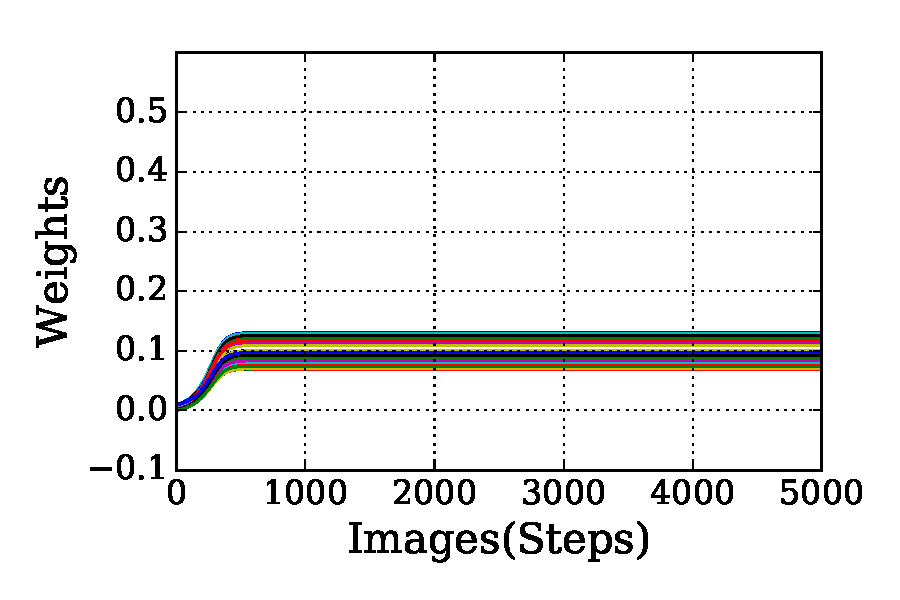
\includegraphics[width=\textwidth]{pics_sdlm/20_exp_AE/exp1_weights_non.pdf}
			\caption{Weights of Exp1}
		\end{subfigure}
		\begin{subfigure}[t]{0.4\textwidth}
			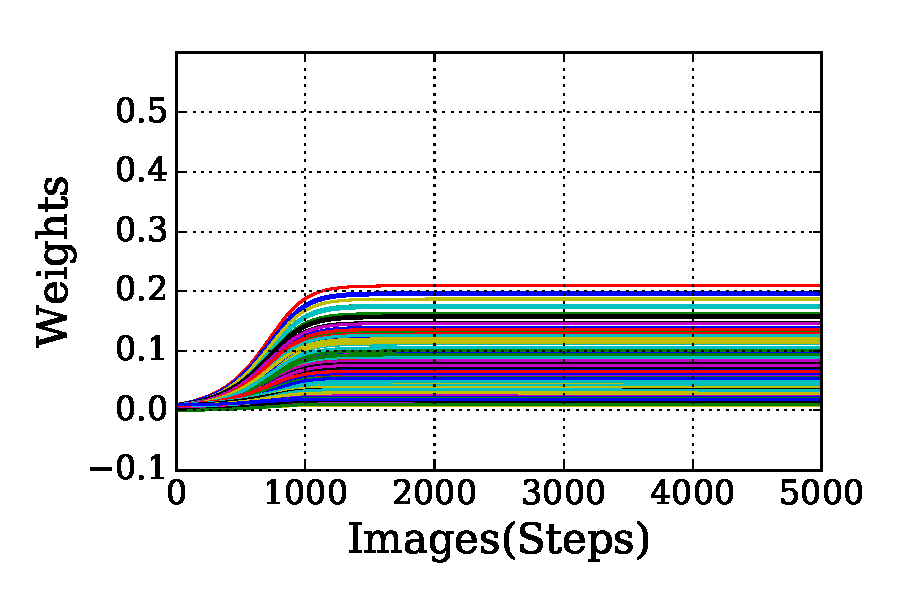
\includegraphics[width=\textwidth]{pics_sdlm/20_exp_AE/exp2_weights_non.pdf}
			\caption{Weights of Exp2}
		\end{subfigure}
		\begin{subfigure}[t]{0.4\textwidth}
			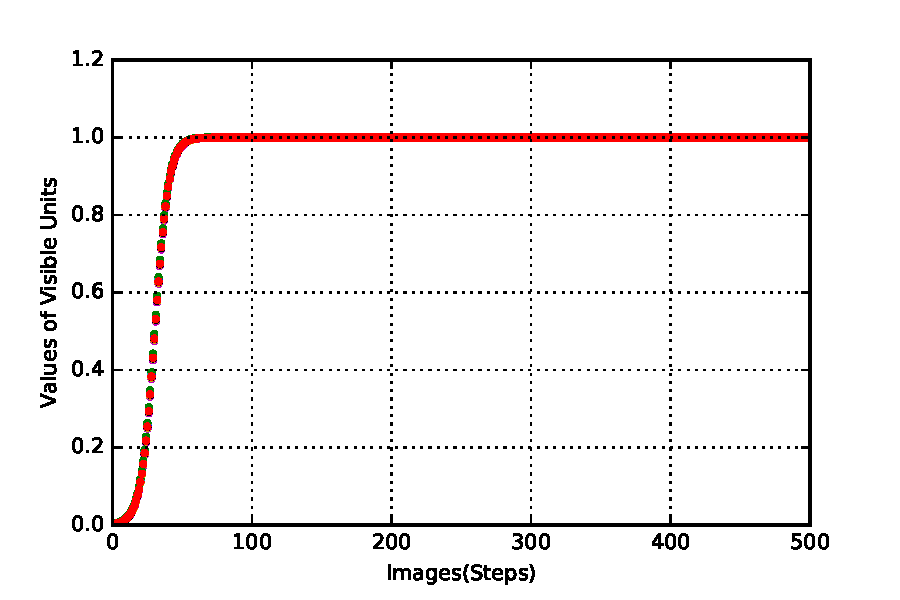
\includegraphics[width=\textwidth]{pics_sdlm/20_exp_AE/exp1_recon_non.pdf}
			\caption{Reconstruction of visible units in Exp1}
		\end{subfigure}
		\begin{subfigure}[t]{0.4\textwidth}
			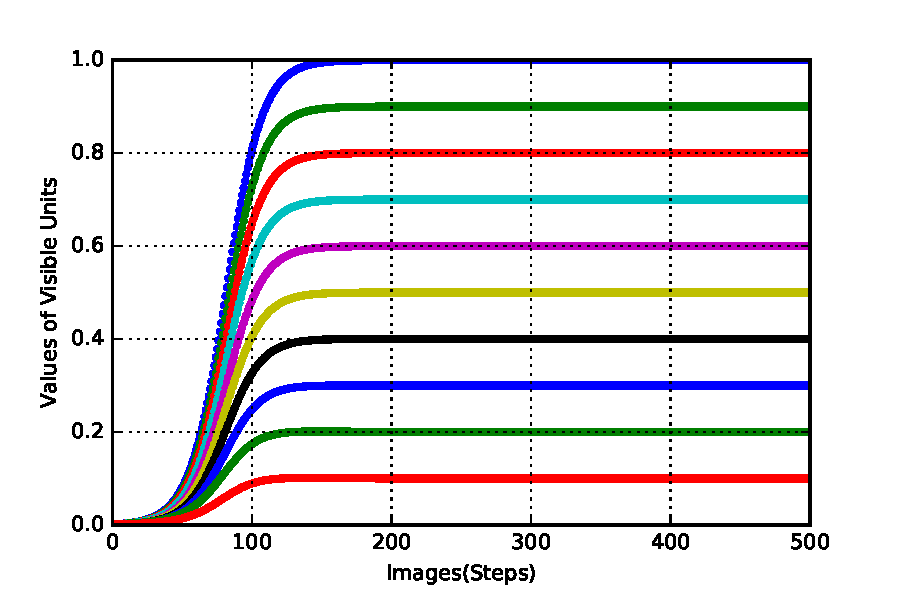
\includegraphics[width=\textwidth]{pics_sdlm/20_exp_AE/exp2_recon_non.pdf}
			\caption{Reconstruction of visible units in Exp2}
		\end{subfigure}\\
		\begin{subfigure}[t]{0.4\textwidth}
			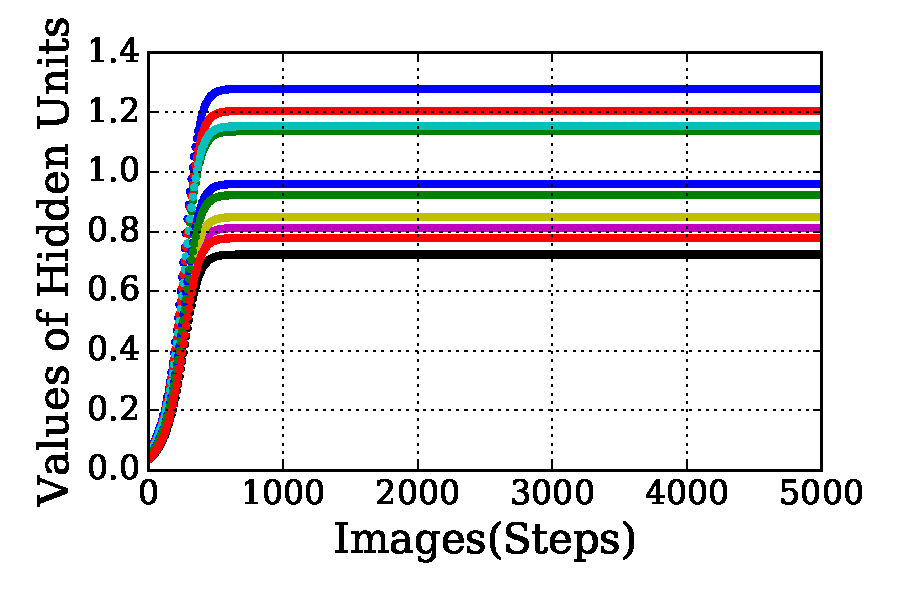
\includegraphics[width=\textwidth]{pics_sdlm/20_exp_AE/exp1_hid_non.pdf}
			\caption{Output of hidden units in Exp1}
		\end{subfigure}
		\begin{subfigure}[t]{0.4\textwidth}
			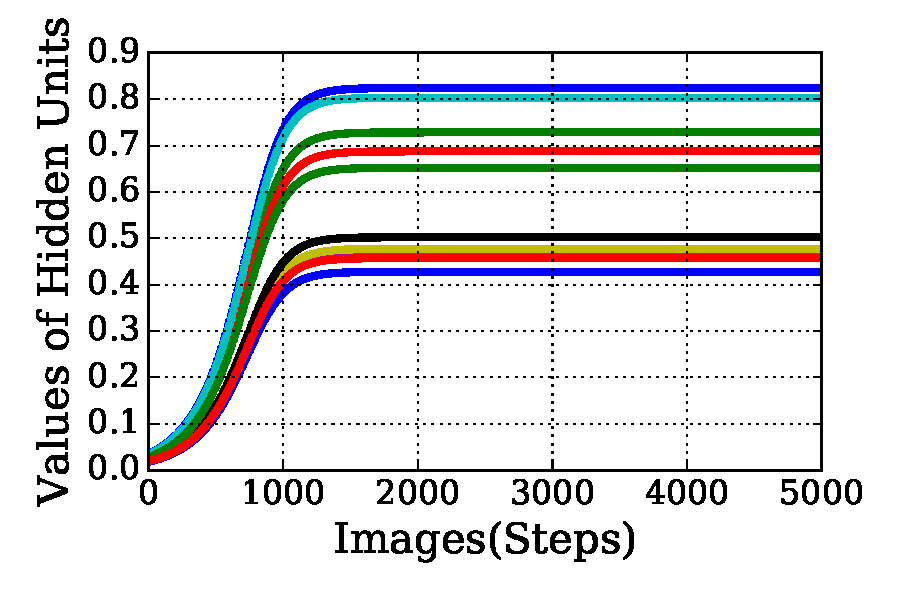
\includegraphics[width=\textwidth]{pics_sdlm/20_exp_AE/exp2_hid_non.pdf}
			\caption{Output of hidden units in Exp2}
		\end{subfigure}\\
		\begin{subfigure}[t]{0.4\textwidth}
			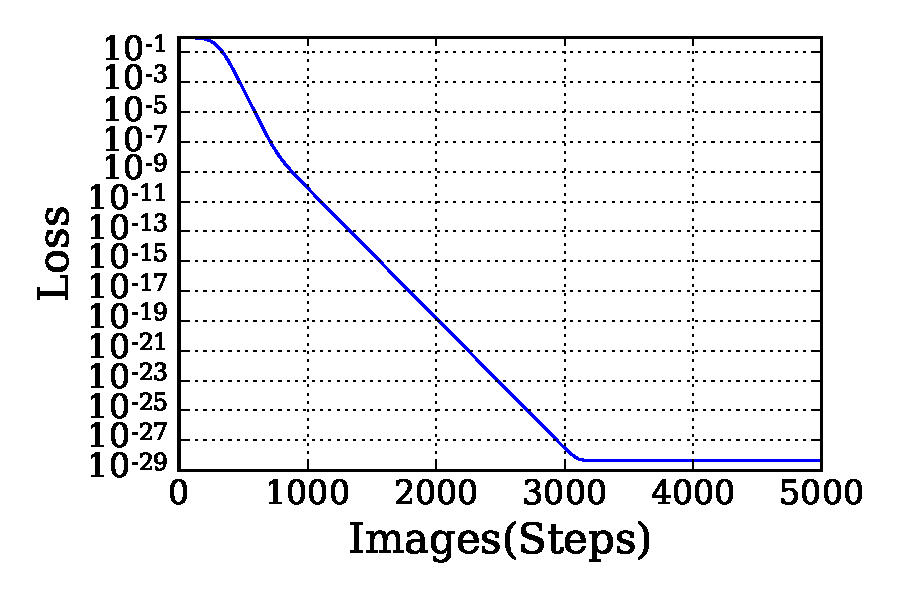
\includegraphics[width=\textwidth]{pics_sdlm/20_exp_AE/exp1_loss.pdf}
			\caption{Output of hidden units in Exp1}
		\end{subfigure}
		\begin{subfigure}[t]{0.4\textwidth}
			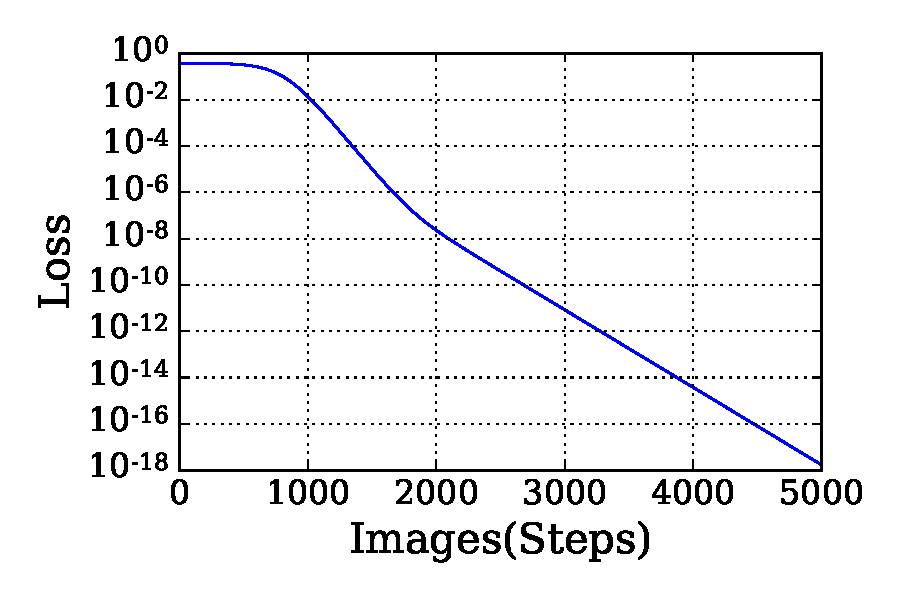
\includegraphics[width=\textwidth]{pics_sdlm/20_exp_AE/exp2_loss.pdf}
			\caption{Output of hidden units in Exp2}
		\end{subfigure}
		\caption{Changes of weights, output of visible and hidden units, and mean squared error (loss) during the AE training of the reconstruction tests. 
			Experiments 1) 10 visible units fully connected to 10 hidden units with input data of all 1s; 2) same network fed with 10 values distribute linearly from 0.1 to 1.}
	\end{figure}



\subsection{Restricted Boltzmann Machine}

Examples of using an autoencoder with 10 input neurons and 10 hidden neurons: reconstruction the input data $\mathbf{v}$ where I) $v_i = 1$, II) $v_i = i/10$.
\begin{figure}
	\centering
	\begin{subfigure}[t]{0.4\textwidth}
		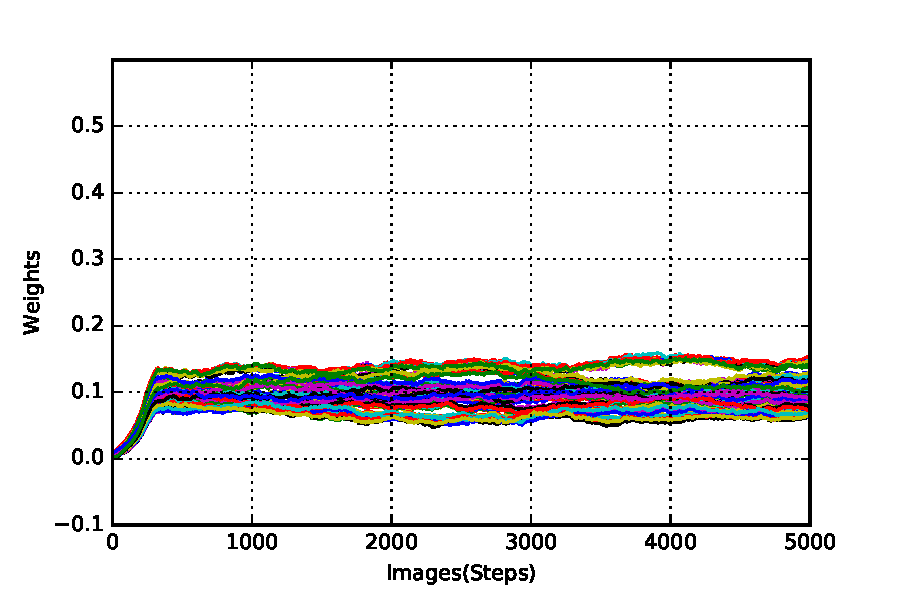
\includegraphics[width=\textwidth]{pics_sdlm/30_exp_RBM/exp1_weights_non.pdf}
		\caption{Weights of Exp1}
	\end{subfigure}
	\begin{subfigure}[t]{0.4\textwidth}
		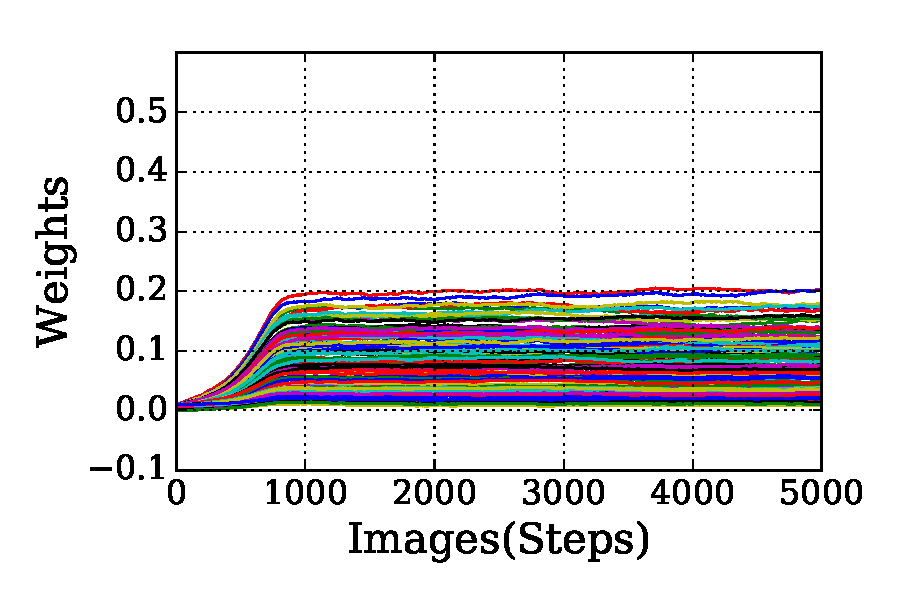
\includegraphics[width=\textwidth]{pics_sdlm/30_exp_RBM/exp2_weights_non.pdf}
		\caption{Weights of Exp2}
	\end{subfigure}
	\begin{subfigure}[t]{0.4\textwidth}
		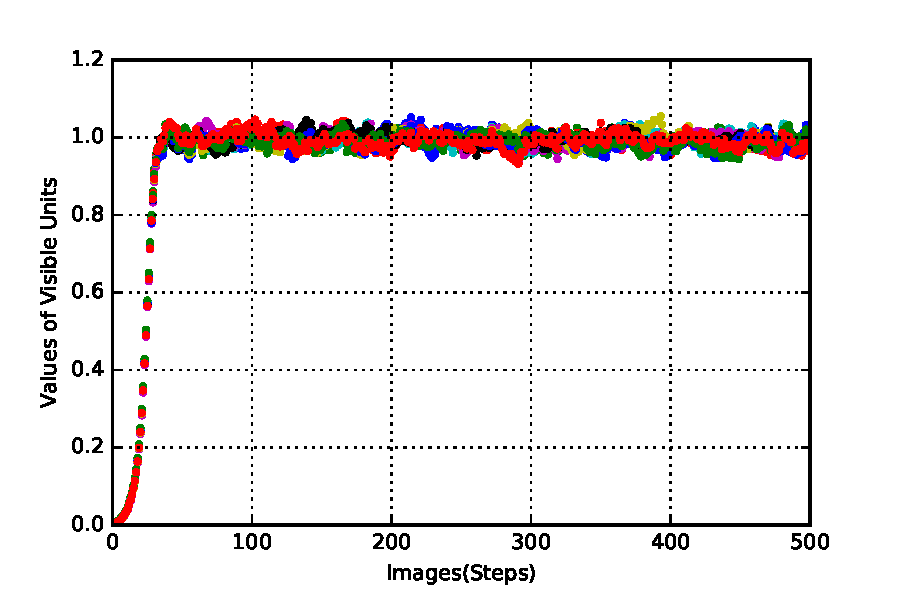
\includegraphics[width=\textwidth]{pics_sdlm/30_exp_RBM/exp1_recon_non.pdf}
		\caption{Reconstruction of visible units in Exp1}
	\end{subfigure}
	\begin{subfigure}[t]{0.4\textwidth}
		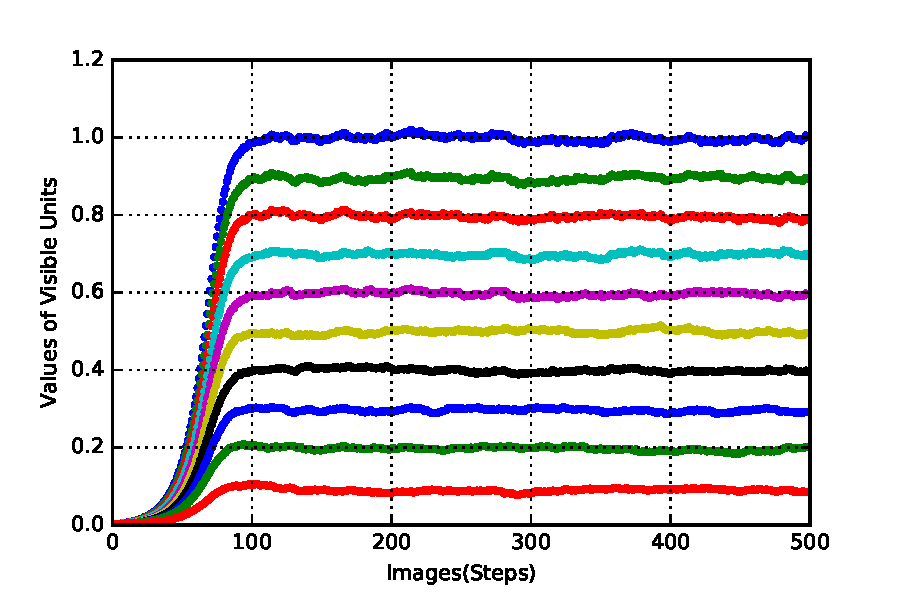
\includegraphics[width=\textwidth]{pics_sdlm/30_exp_RBM/exp2_recon_non.pdf}
		\caption{Reconstruction of visible units in Exp2}
	\end{subfigure}\\
	\begin{subfigure}[t]{0.4\textwidth}
		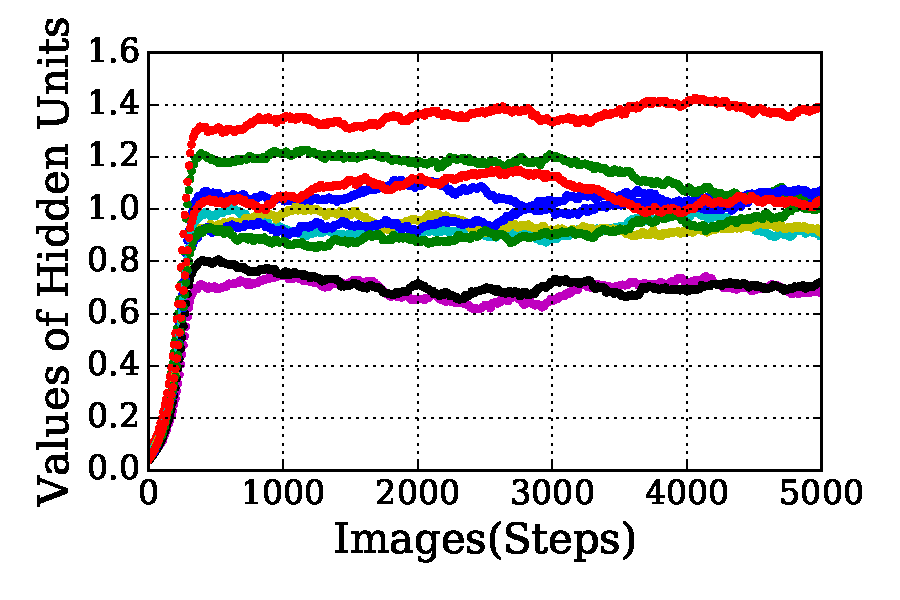
\includegraphics[width=\textwidth]{pics_sdlm/30_exp_RBM/exp1_hid_non.pdf}
		\caption{Output of hidden units in Exp1}
	\end{subfigure}
	\begin{subfigure}[t]{0.4\textwidth}
		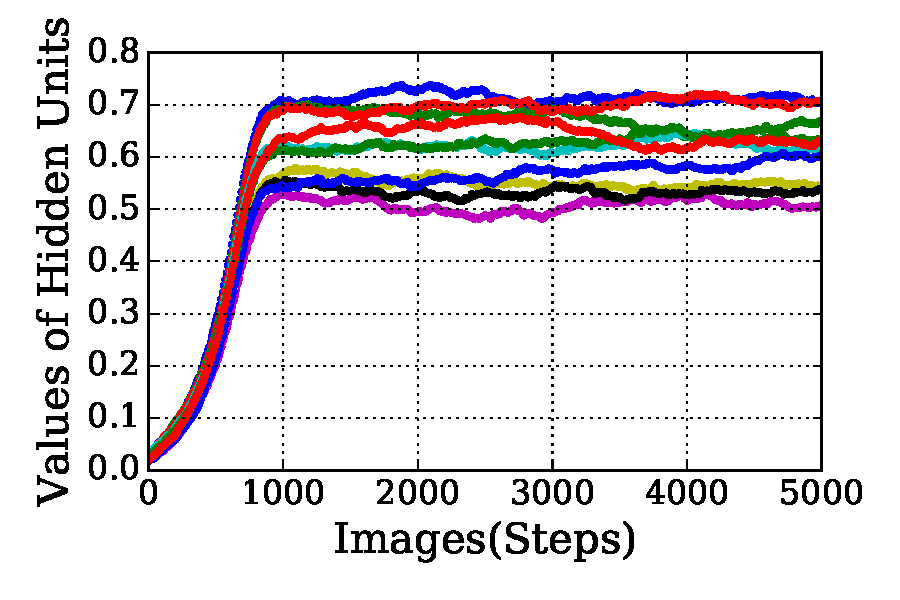
\includegraphics[width=\textwidth]{pics_sdlm/30_exp_RBM/exp2_hid_non.pdf}
		\caption{Output of hidden units in Exp2}
	\end{subfigure}\\
	\begin{subfigure}[t]{0.4\textwidth}
		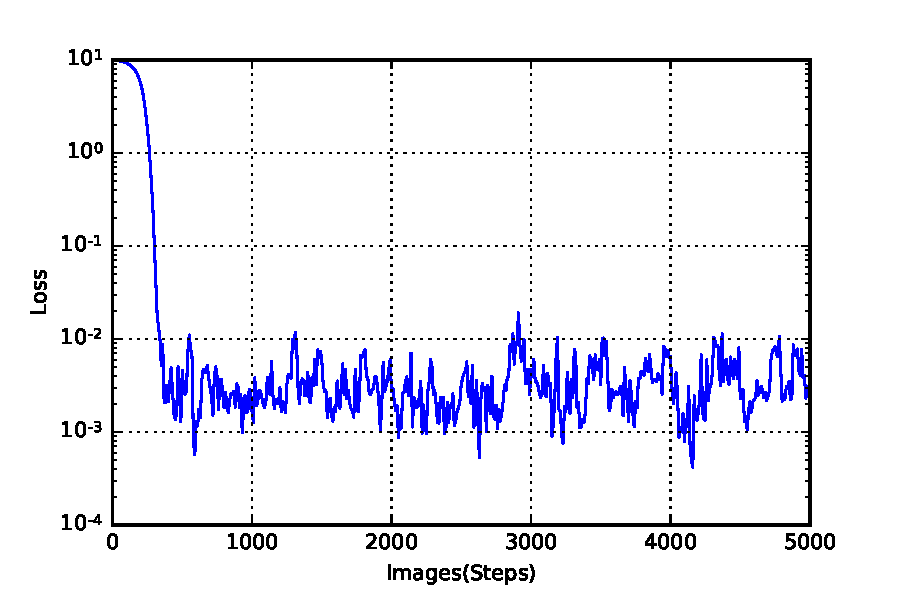
\includegraphics[width=\textwidth]{pics_sdlm/30_exp_RBM/exp1_loss.pdf}
		\caption{Output of hidden units in Exp1}
	\end{subfigure}
	\begin{subfigure}[t]{0.4\textwidth}
		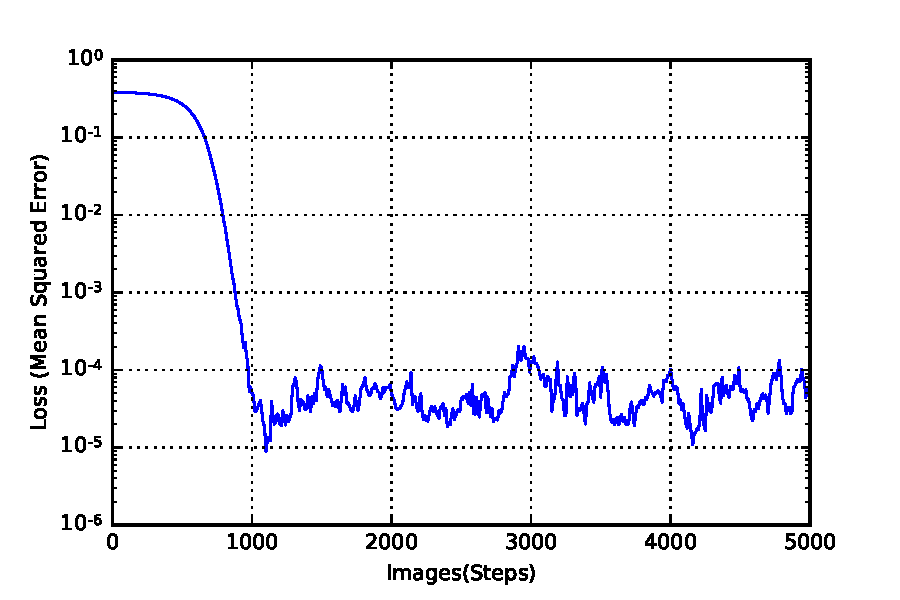
\includegraphics[width=\textwidth]{pics_sdlm/30_exp_RBM/exp2_loss.pdf}
		\caption{Output of hidden units in Exp2}
	\end{subfigure}
	\caption{Changes of weights, output of visible and hidden units, and mean squared error (loss) during the nRBM training of the reconstruction tests. 
		Experiments 1) 10 visible units fully connected to 10 hidden units with input data of all 1s; 2) same network fed with 10 values distribute linearly from 0.1 to 1.}
\end{figure}

\section{Biologically Plausible Training}
\subsection{Rate-based coding}
The encoding method is the same as stated below in Chapter~\ref{sec:poissonian}.
It introduces noise to the original input.
The experiments on noisy input driven by Poissonian spike trains.
Figure~\ref{fig:poisson_ae} and Figure~\ref{fig:poisson_rbm} show how noise influence the training and output of both the visible and hidden units.
The change of the weights oscillates more. % and the value of the weights tends to diverge slightly as training goes on. 
The experiments run as a baseline to compare with spike based training in the following Section.
\begin{figure}
	\centering
	\begin{subfigure}[t]{0.4\textwidth}
		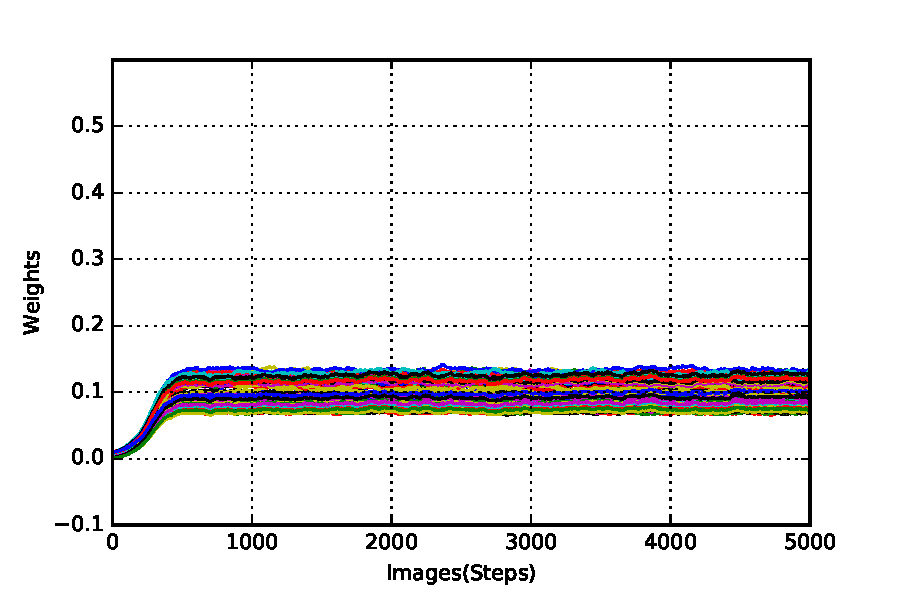
\includegraphics[width=\textwidth]{pics_sdlm/21_exp_AE_noise/exp1_weights_s.pdf}
		\caption{Weights of Exp1}
	\end{subfigure}
	\begin{subfigure}[t]{0.4\textwidth}
		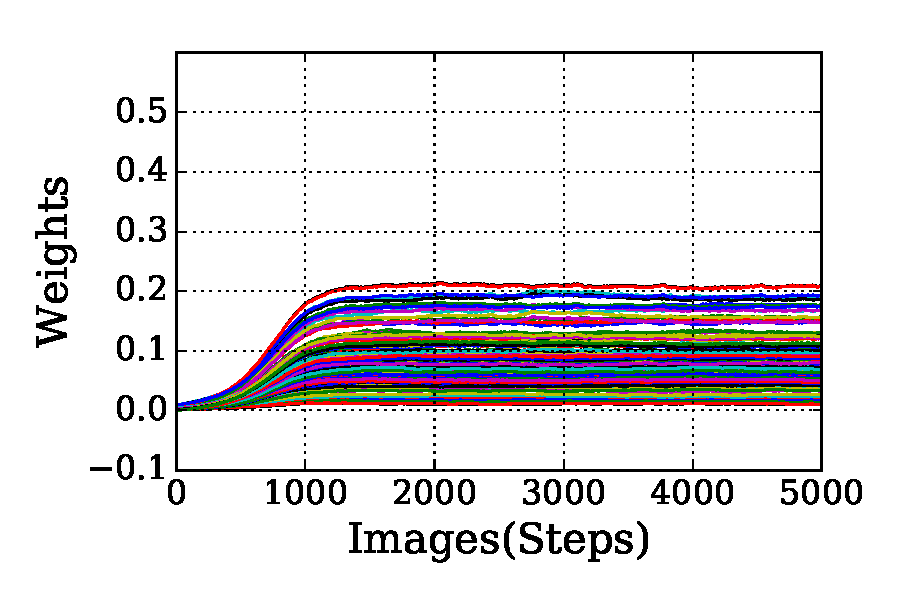
\includegraphics[width=\textwidth]{pics_sdlm/21_exp_AE_noise/exp2_weights_s.pdf}
		\caption{Weights of Exp2}
	\end{subfigure}
	\begin{subfigure}[t]{0.4\textwidth}
		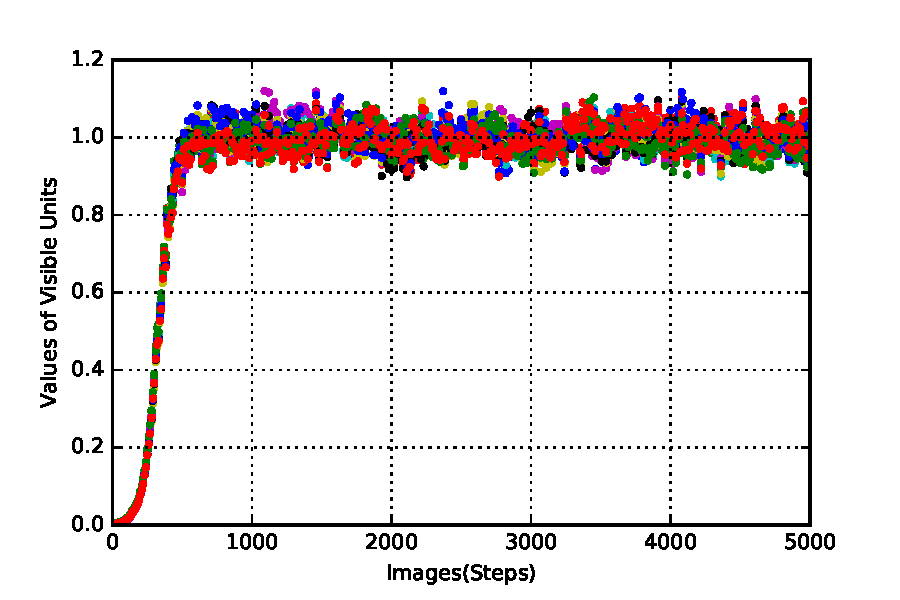
\includegraphics[width=\textwidth]{pics_sdlm/21_exp_AE_noise/exp1_recon_s.pdf}
		\caption{Reconstruction of visible units in Exp1}
	\end{subfigure}
	\begin{subfigure}[t]{0.4\textwidth}
		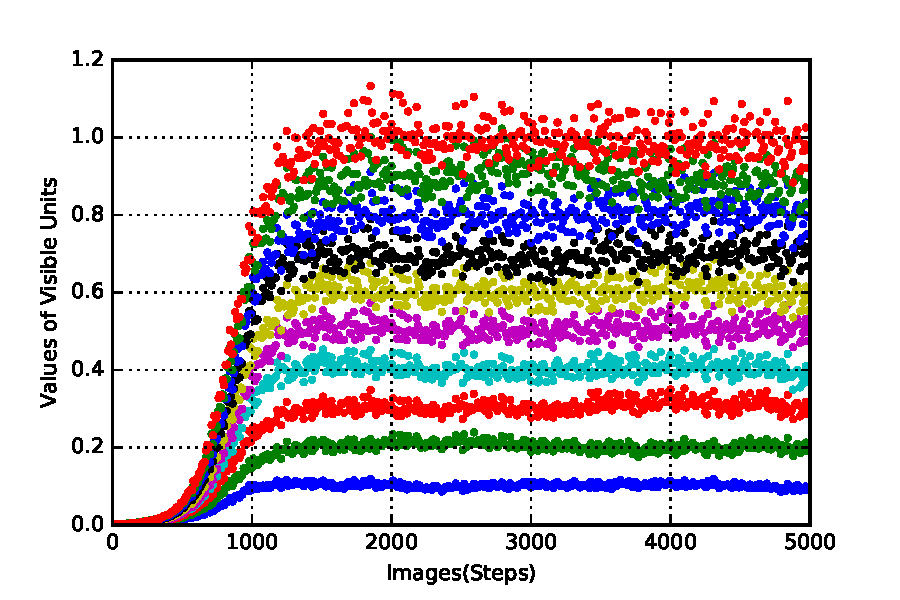
\includegraphics[width=\textwidth]{pics_sdlm/21_exp_AE_noise/exp2_recon_s.pdf}
		\caption{Reconstruction of visible units in Exp2}
	\end{subfigure}\\
	\begin{subfigure}[t]{0.4\textwidth}
		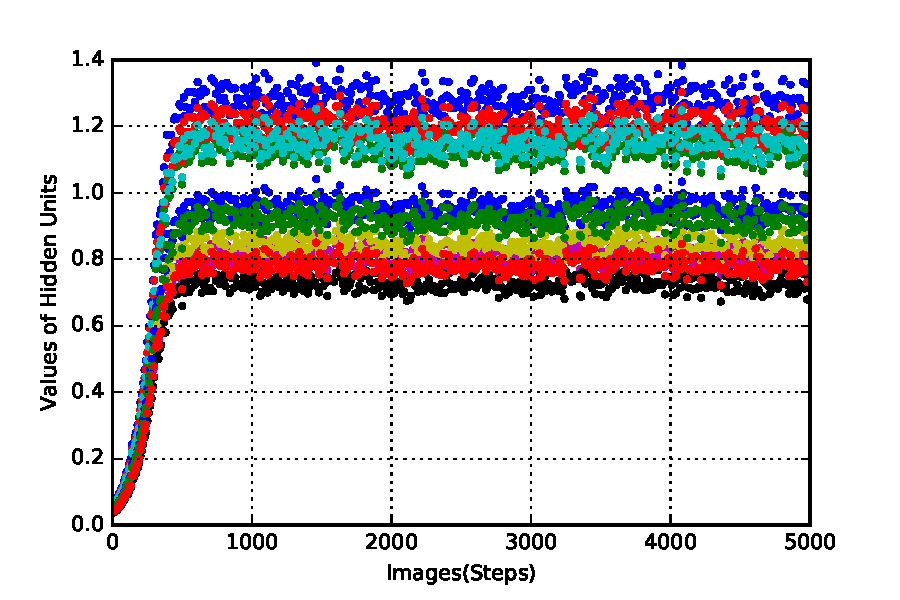
\includegraphics[width=\textwidth]{pics_sdlm/21_exp_AE_noise/exp1_hid_s.pdf}
		\caption{Output of hidden units in Exp1}
	\end{subfigure}
	\begin{subfigure}[t]{0.4\textwidth}
		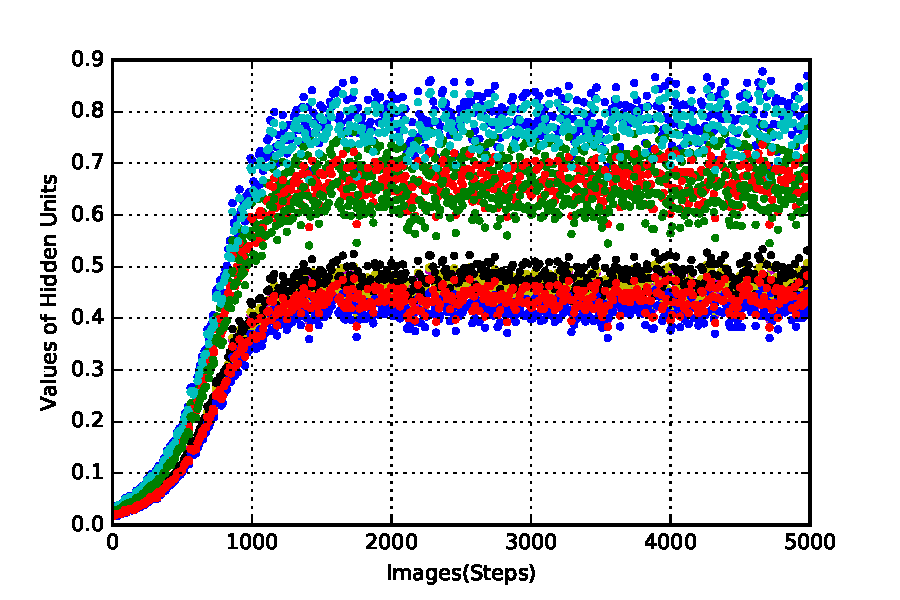
\includegraphics[width=\textwidth]{pics_sdlm/21_exp_AE_noise/exp2_hid_s.pdf}
		\caption{Output of hidden units in Exp2}
	\end{subfigure}\\
	\begin{subfigure}[t]{0.4\textwidth}
		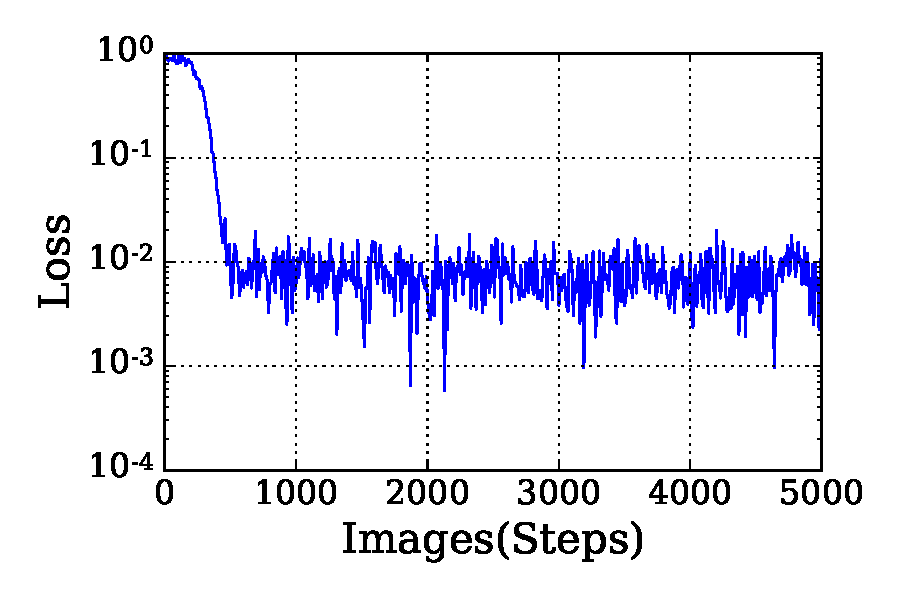
\includegraphics[width=\textwidth]{pics_sdlm/21_exp_AE_noise/exp1_loss_s.pdf}
		\caption{Output of hidden units in Exp1}
	\end{subfigure}
	\begin{subfigure}[t]{0.4\textwidth}
		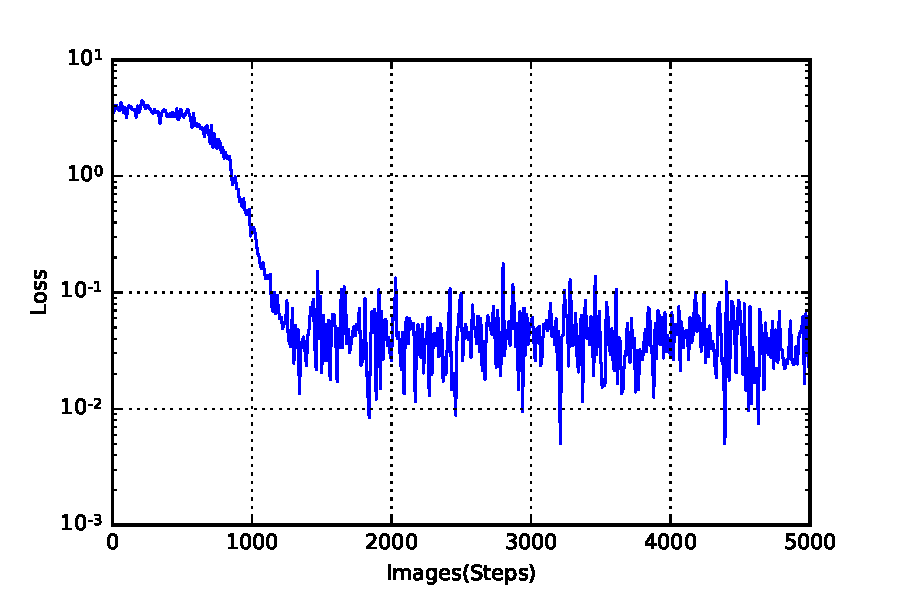
\includegraphics[width=\textwidth]{pics_sdlm/21_exp_AE_noise/exp2_loss_s.pdf}
		\caption{Output of hidden units in Exp2}
	\end{subfigure}
	\caption{Changes of weights, output of visible and hidden units, and mean squared error (loss) during the AE training of the reconstruction tests. 
		Experiments 1) 10 visible units fully connected to 10 hidden units with the count of Poisson spikes firing at 100~Hz which lasted 100~ms; 2) same network fed with 10 count of Poisson spikes at firing rate ranging from 10~Hz to 100~Hz.}
	\label{fig:poisson_ae}
\end{figure}

\begin{figure}
	\centering
	\begin{subfigure}[t]{0.4\textwidth}
		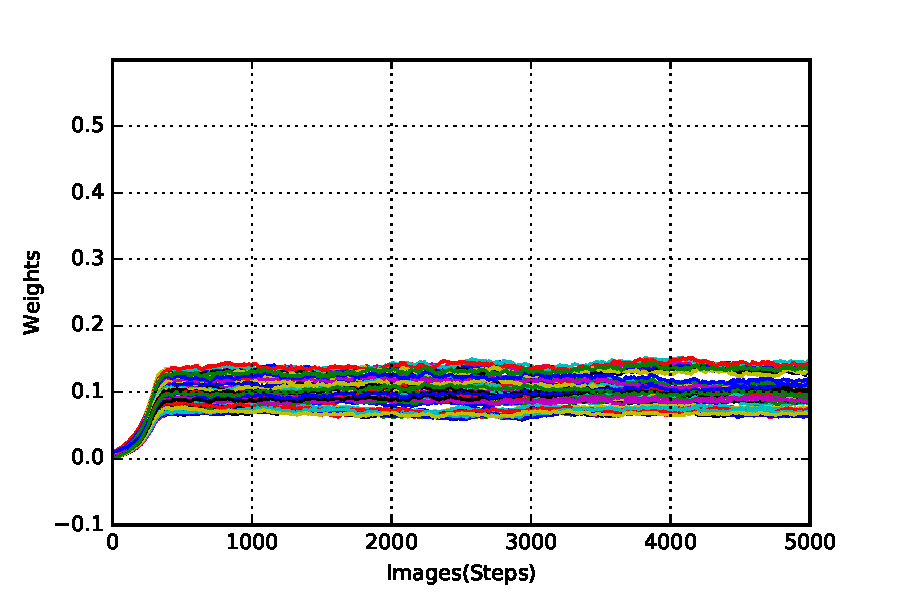
\includegraphics[width=\textwidth]{pics_sdlm/31_exp_RBM_noise/exp1_weights_s.pdf}
		\caption{Weights of Exp1}
	\end{subfigure}
	\begin{subfigure}[t]{0.4\textwidth}
		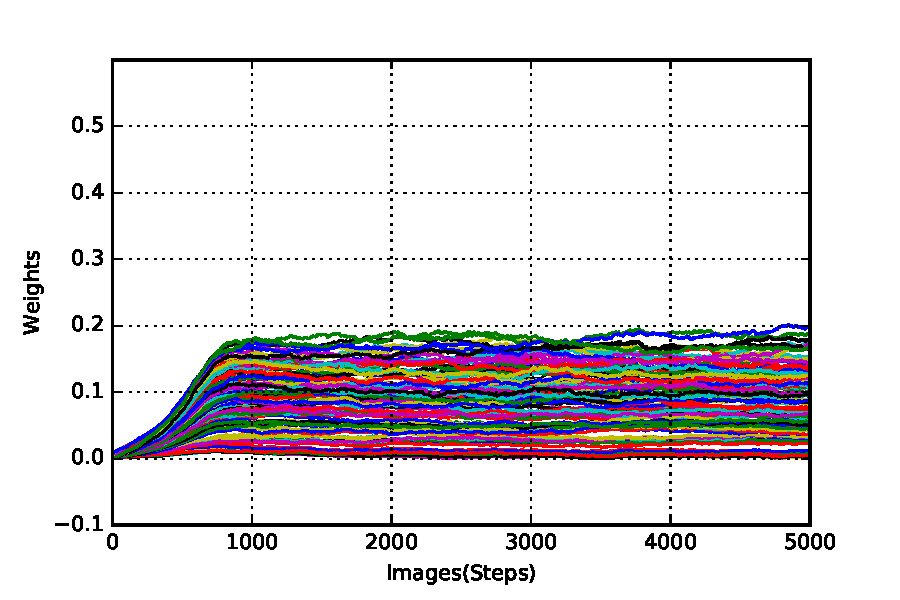
\includegraphics[width=\textwidth]{pics_sdlm/31_exp_RBM_noise/exp2_weights_s.pdf}
		\caption{Weights of Exp2}
	\end{subfigure}
	\begin{subfigure}[t]{0.4\textwidth}
		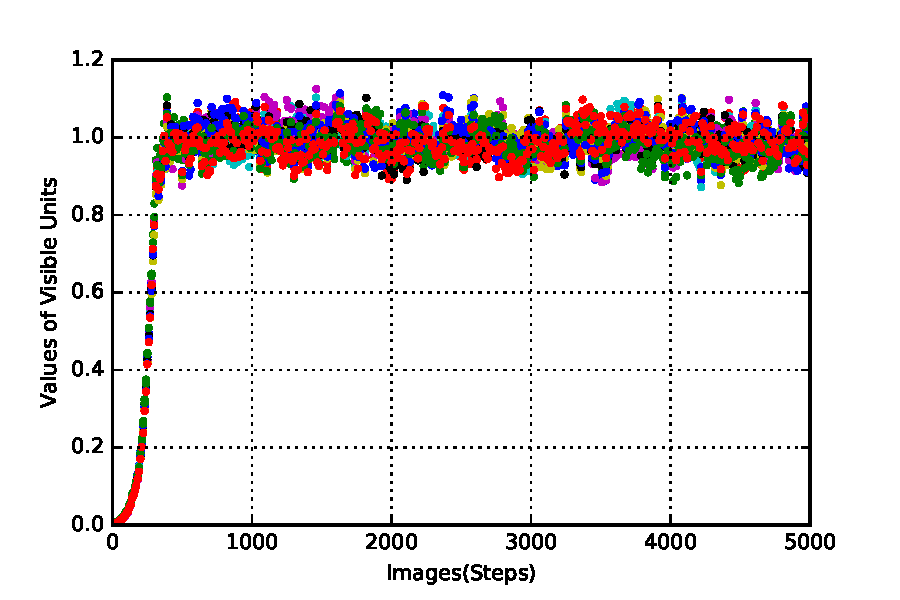
\includegraphics[width=\textwidth]{pics_sdlm/31_exp_RBM_noise/exp1_recon_s.pdf}
		\caption{Reconstruction of visible units in Exp1}
	\end{subfigure}
	\begin{subfigure}[t]{0.4\textwidth}
		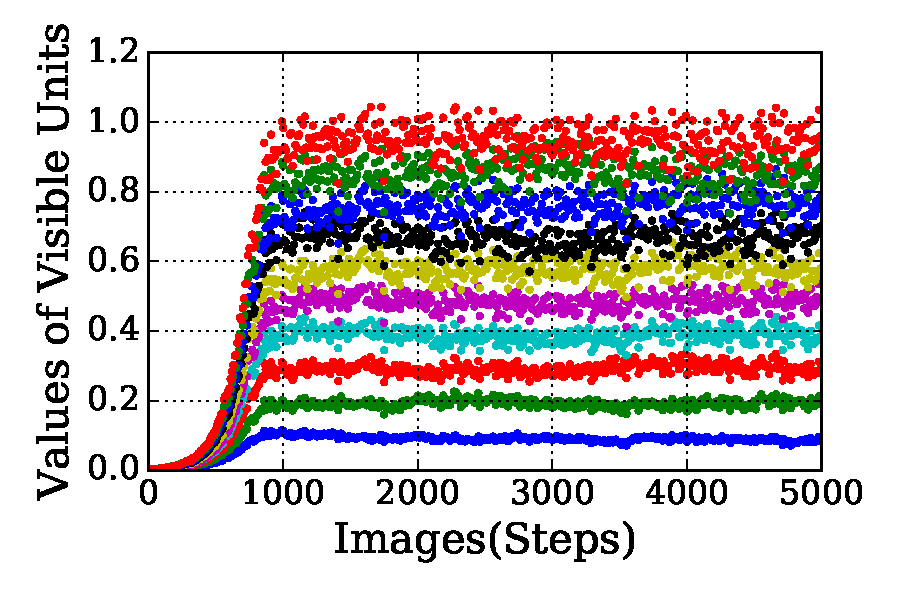
\includegraphics[width=\textwidth]{pics_sdlm/31_exp_RBM_noise/exp2_recon_s.pdf}
		\caption{Reconstruction of visible units in Exp2}
	\end{subfigure}\\
	\begin{subfigure}[t]{0.4\textwidth}
		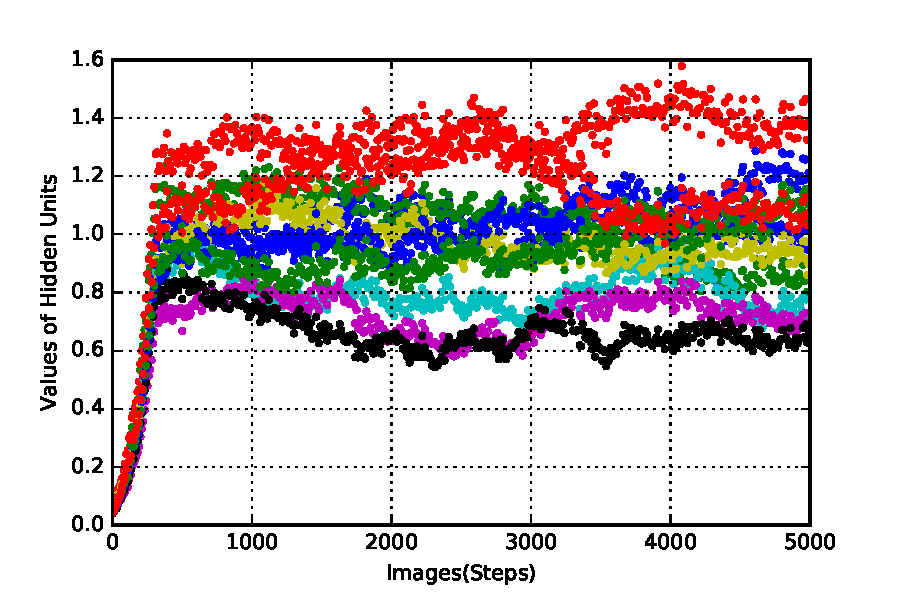
\includegraphics[width=\textwidth]{pics_sdlm/31_exp_RBM_noise/exp1_hid_s.pdf}
		\caption{Output of hidden units in Exp1}
	\end{subfigure}
	\begin{subfigure}[t]{0.4\textwidth}
		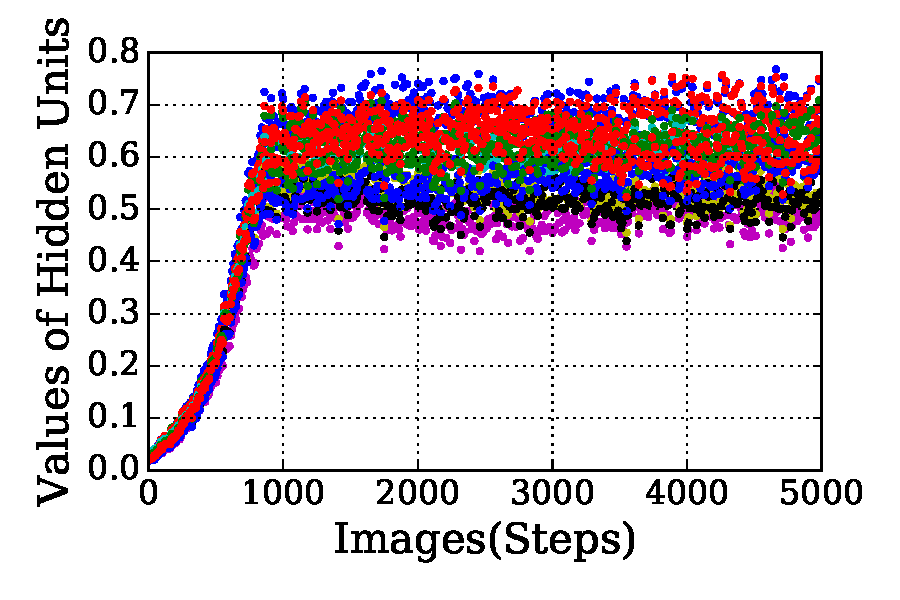
\includegraphics[width=\textwidth]{pics_sdlm/31_exp_RBM_noise/exp2_hid_s.pdf}
		\caption{Output of hidden units in Exp2}
	\end{subfigure}\\
	\begin{subfigure}[t]{0.4\textwidth}
		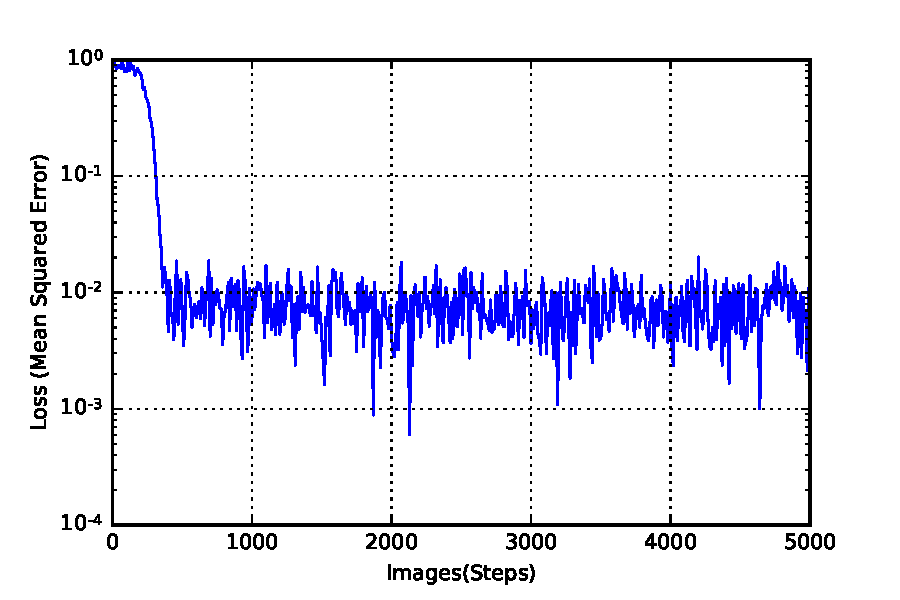
\includegraphics[width=\textwidth]{pics_sdlm/31_exp_RBM_noise/exp1_loss_s.pdf}
		\caption{Output of hidden units in Exp1}
	\end{subfigure}
	\begin{subfigure}[t]{0.4\textwidth}
		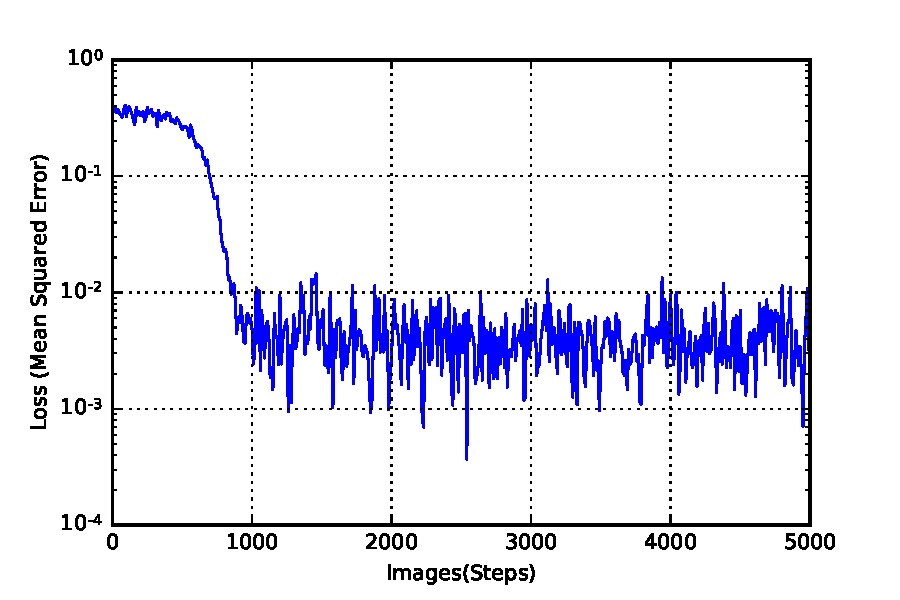
\includegraphics[width=\textwidth]{pics_sdlm/31_exp_RBM_noise/exp2_loss_s.pdf}
		\caption{Output of hidden units in Exp2}
	\end{subfigure}
	\caption{Changes of weights, output of visible and hidden units, and mean squared error (loss) during the nRBM training of the reconstruction tests. 
		Experiments 1) 10 visible units fully connected to 10 hidden units with the count of Poisson spikes firing at 100~Hz which lasted 100~ms; 2) same network fed with 10 count of Poisson spikes at firing rate ranging from 10~Hz to 100~Hz.}
	\label{fig:poisson_rbm}
\end{figure}

\subsection{STDP}

\subsection{Training Spiking Autoencoders}
Rate-based learning of STDP (rSTDP) which is inspired by ReSuMe.
Biology, local\\
-Why it works stated in Maths.\\
\begin{equation}
\begin{aligned}
\overline{\Delta w_{ij}} &\propto \eta \lambda_{h_i}(\lambda_{v_j} - \lambda_{v'_j})\\
&=\eta'P_{h_i}P_{v_j}\tau_{w} \tau_{dur} - \eta'P_{h_i}P_{v'_j}\tau_{w} \tau_{dur}, \textrm{where,}\\
P_{s} &= \lambda_{s} \times 0.001~s = \frac{K s}{1000}\\
\eta' &= \frac{10^6}{K^2 \tau_{w} \tau_{dur}} \eta
\end{aligned}
\end{equation}
\begin{figure}
	\centering
	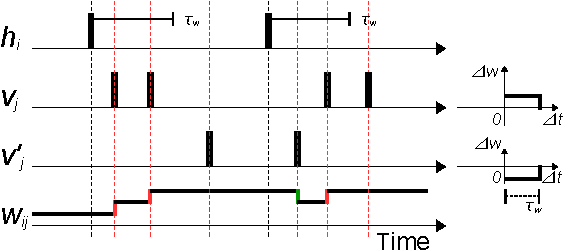
\includegraphics[width=0.8\textwidth]{pics_sdlm/rSTDP.pdf}
	\caption{How rSTDP works in training spiking Autoencoders.}
	\label{fig:rSTDP}
\end{figure}

\subsection{Training Spiking RBM}
\begin{figure}
	\centering
	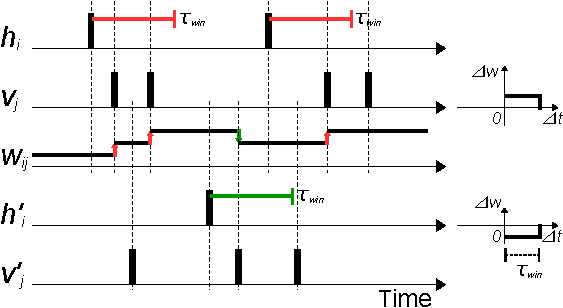
\includegraphics[width=0.8\textwidth]{pics_sdlm/rSTDP_rbm.pdf}
	\caption{How rSTDP works in training spiking RBMs.}
	\label{fig:rSTDP_rbm}
\end{figure}

\section{Problem}
Correlations in spike trains make weights diverge.
Experiments
\begin{figure}
	\centering
	\begin{subfigure}[t]{0.4\textwidth}
		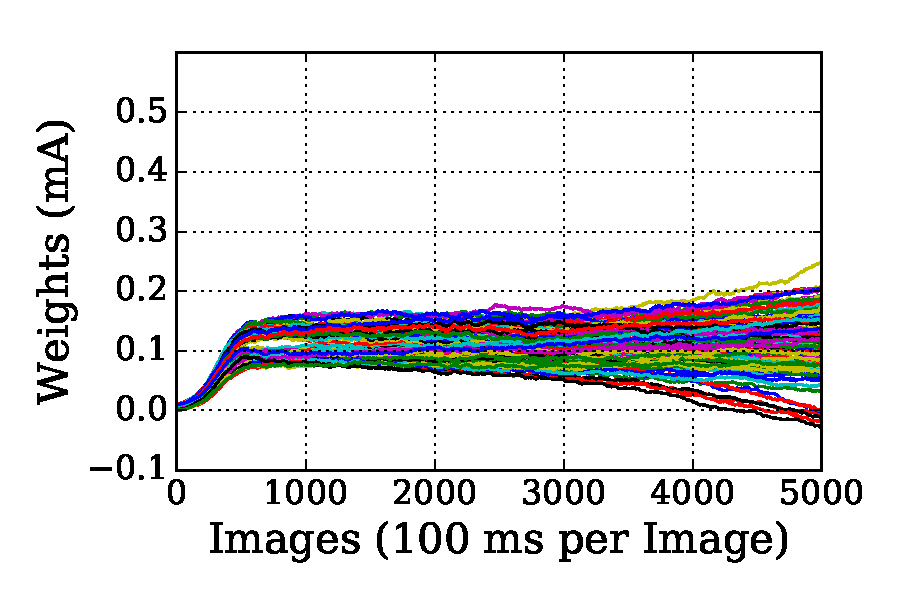
\includegraphics[width=\textwidth]{pics_sdlm/00_exp_SAE_Orig/exp1_weights_s.pdf}
		\caption{Weights of Exp1}
	\end{subfigure}
	\begin{subfigure}[t]{0.4\textwidth}
		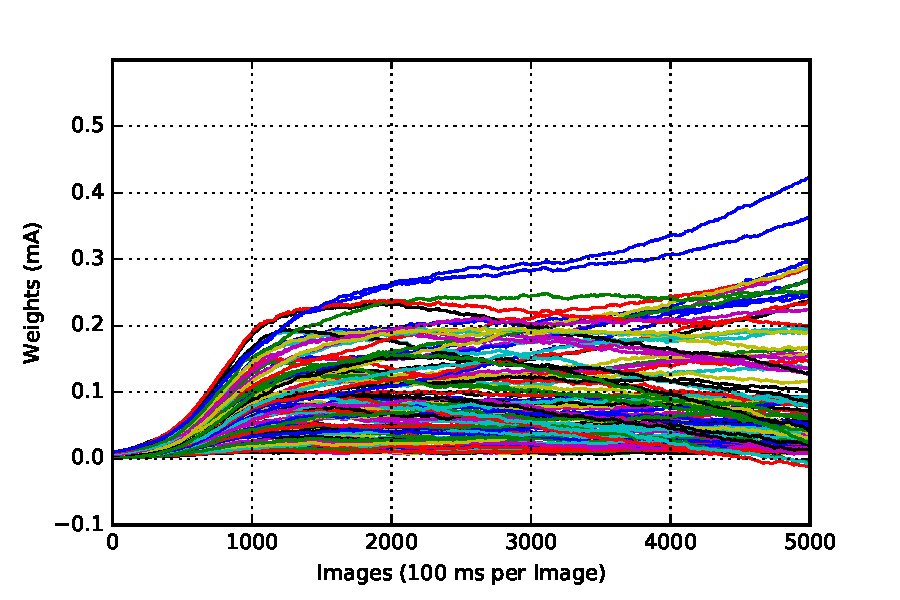
\includegraphics[width=\textwidth]{pics_sdlm/00_exp_SAE_Orig/exp2_weights_s.pdf}
		\caption{Weights of Exp2}
	\end{subfigure}
	\begin{subfigure}[t]{0.4\textwidth}
		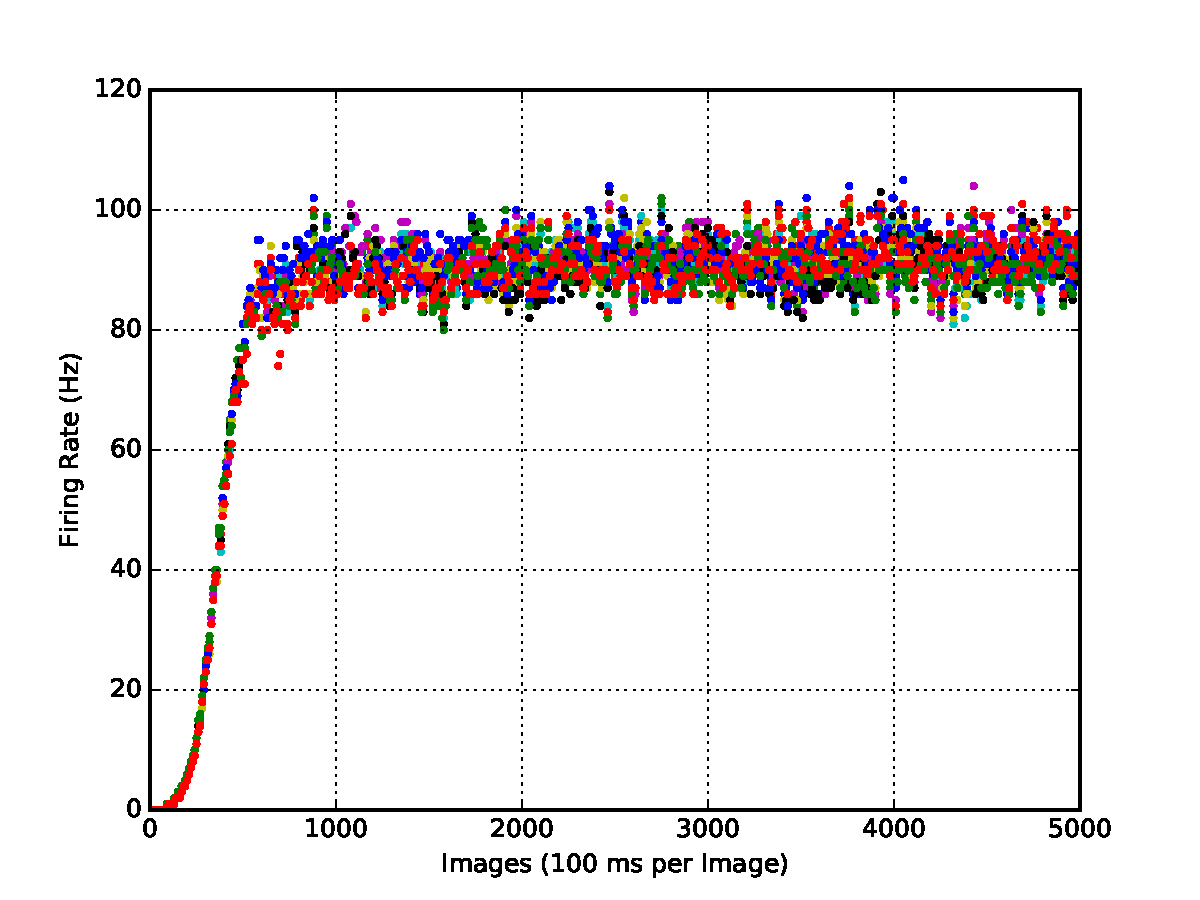
\includegraphics[width=\textwidth]{pics_sdlm/00_exp_SAE_Orig/exp1_recon_s.pdf}
		\caption{Reconstruction of visible units in Exp1}
	\end{subfigure}
	\begin{subfigure}[t]{0.4\textwidth}
		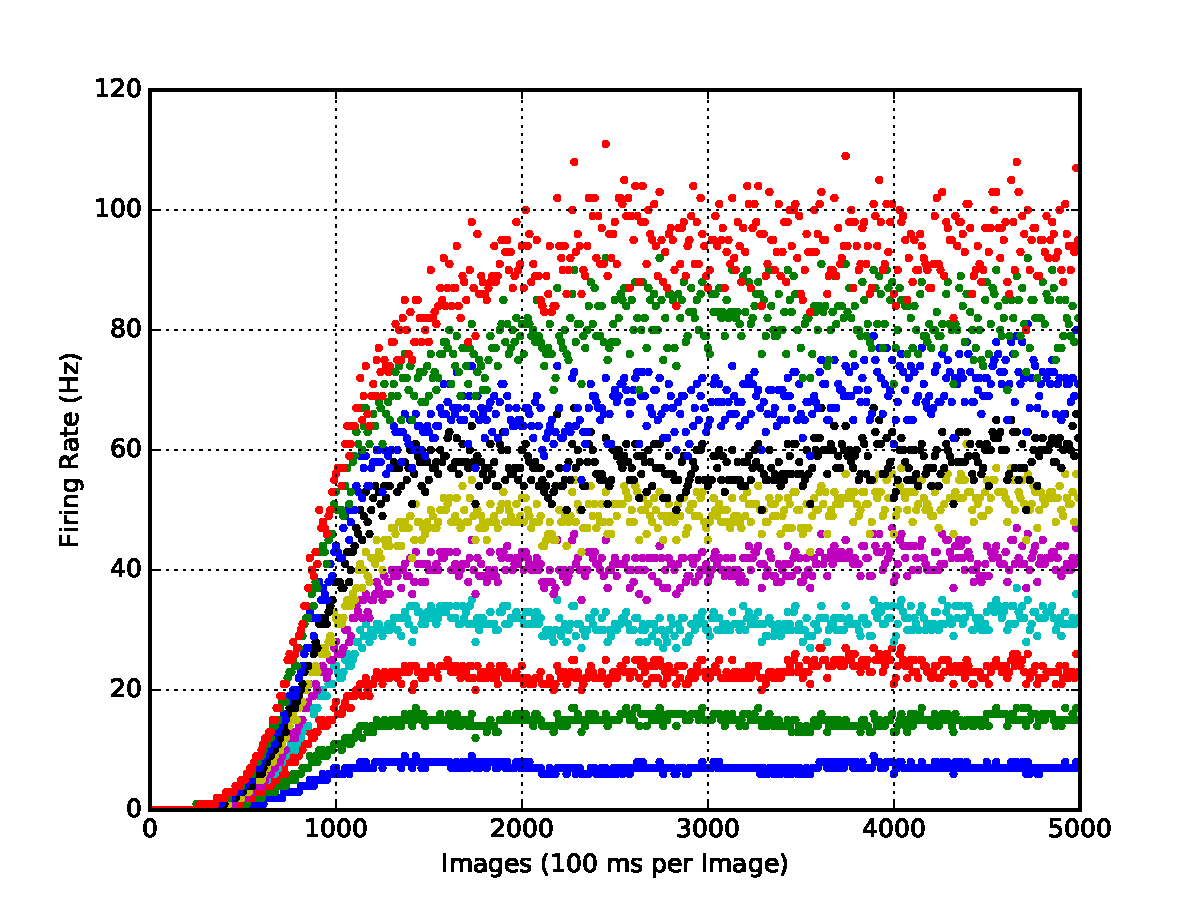
\includegraphics[width=\textwidth]{pics_sdlm/00_exp_SAE_Orig/exp2_recon_s.pdf}
		\caption{Reconstruction of visible units in Exp2}
	\end{subfigure}\\
	\begin{subfigure}[t]{0.4\textwidth}
		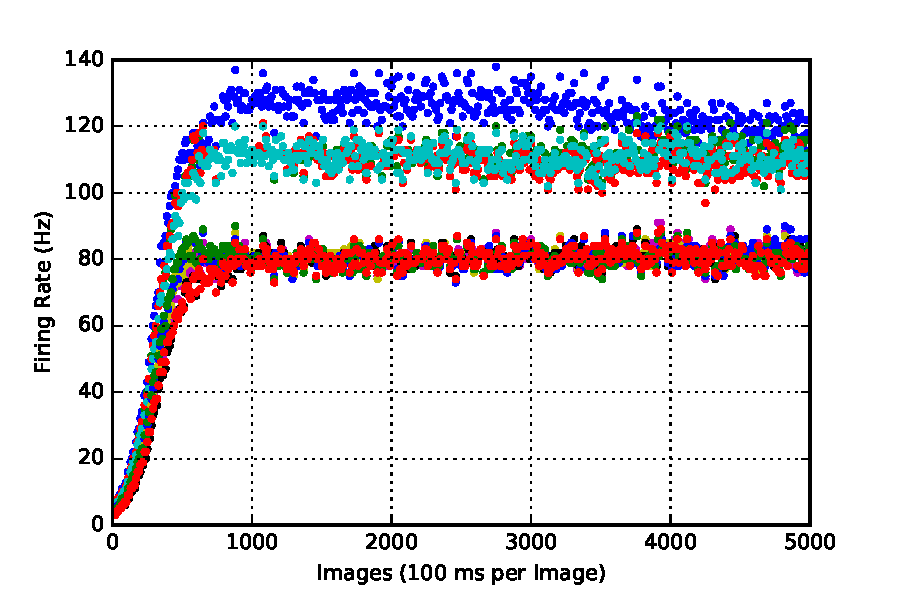
\includegraphics[width=\textwidth]{pics_sdlm/00_exp_SAE_Orig/exp1_hid_s.pdf}
		\caption{Output of hidden units in Exp1}
	\end{subfigure}
	\begin{subfigure}[t]{0.4\textwidth}
		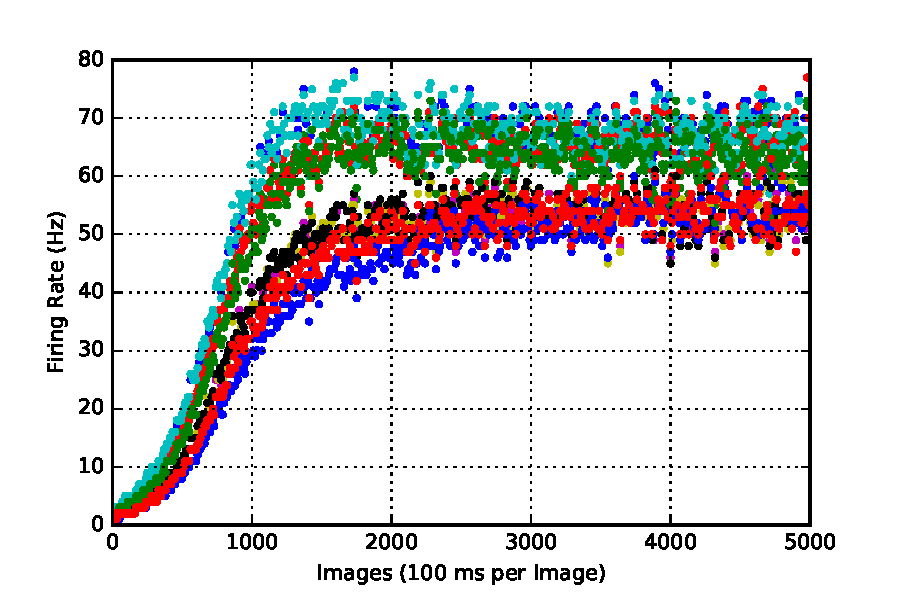
\includegraphics[width=\textwidth]{pics_sdlm/00_exp_SAE_Orig/exp2_hid_s.pdf}
		\caption{Output of hidden units in Exp2}
	\end{subfigure}\\
	\begin{subfigure}[t]{0.4\textwidth}
		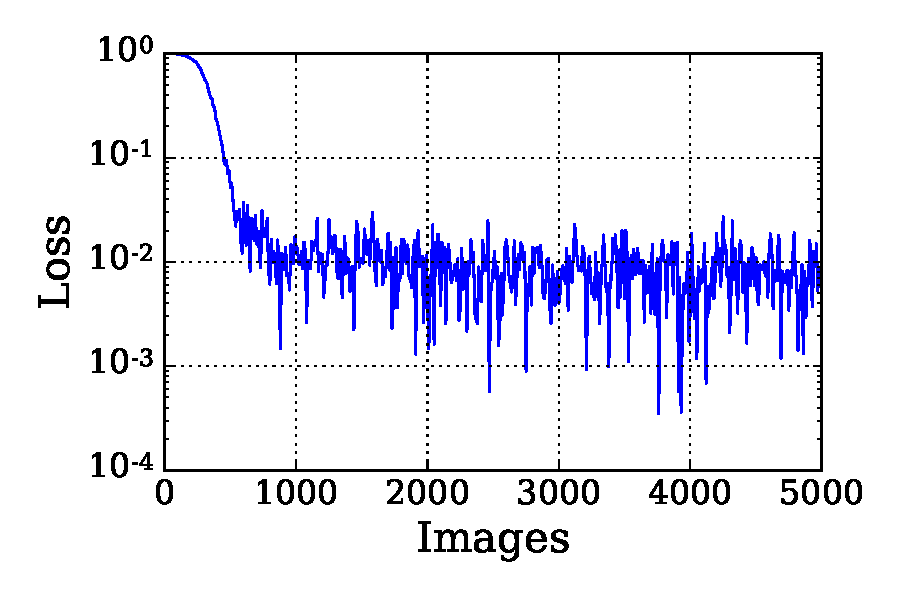
\includegraphics[width=\textwidth]{pics_sdlm/00_exp_SAE_Orig/exp1_mse_nons.pdf}
		\caption{Loss of Exp1}
	\end{subfigure}
	\begin{subfigure}[t]{0.4\textwidth}
		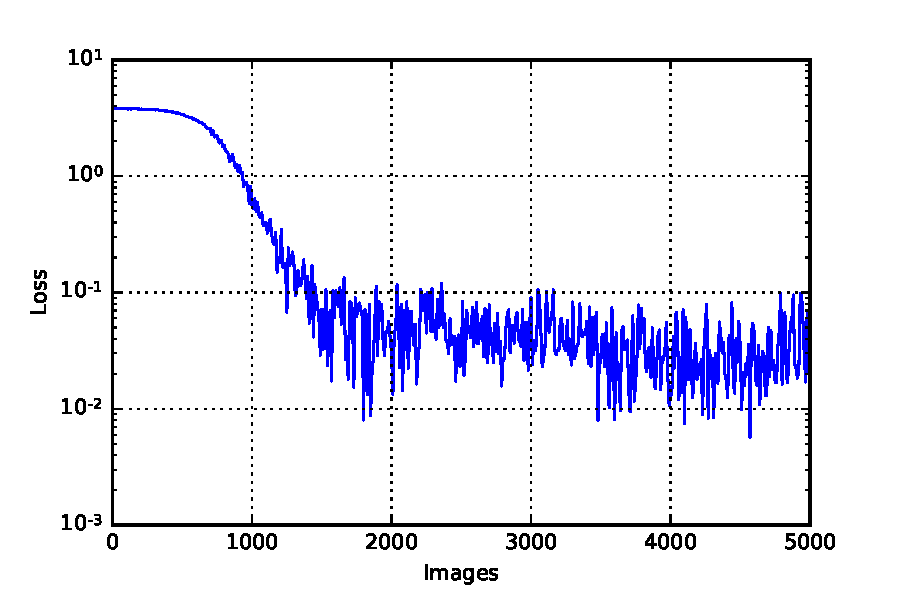
\includegraphics[width=\textwidth]{pics_sdlm/00_exp_SAE_Orig/exp2_mse_nons.pdf}
		\caption{Loss of Exp2}
	\end{subfigure}
	\caption{Weights and firing rates of visible and hidden units change during training of the reconstruction tests of spiking AE. 
		Experiments 1) 10 visible units fully connected to 10 hidden units with Poisson spike trains of 100~Hz which lasted 100~ms; 2) same network fed with 10 Poisson spike trains of firing rate ranging from 10~Hz to 100~Hz.}
\end{figure}

\begin{figure}
	\centering
	\begin{subfigure}[t]{0.4\textwidth}
		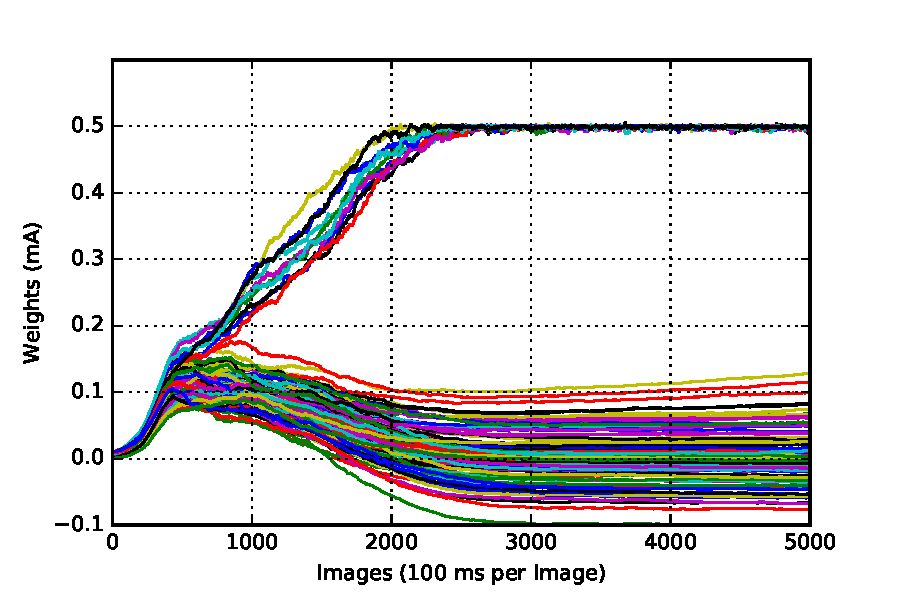
\includegraphics[width=\textwidth]{pics_sdlm/10_exp_SRBM_Orig/exp1_weights_s.pdf}
		\caption{Weights of Exp1}
	\end{subfigure}
	\begin{subfigure}[t]{0.4\textwidth}
		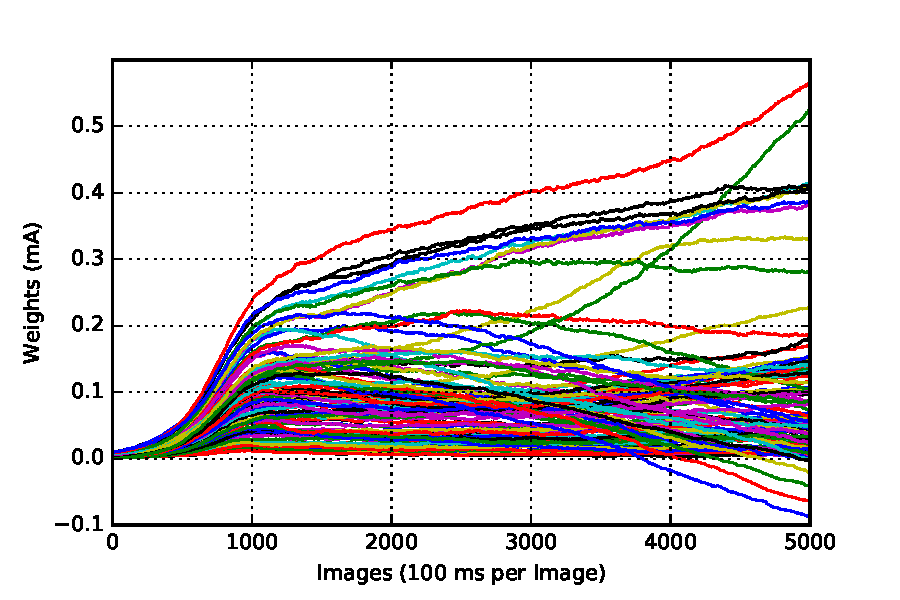
\includegraphics[width=\textwidth]{pics_sdlm/10_exp_SRBM_Orig/exp2_weights_s.pdf}
		\caption{Weights of Exp2}
	\end{subfigure}
	\begin{subfigure}[t]{0.4\textwidth}
		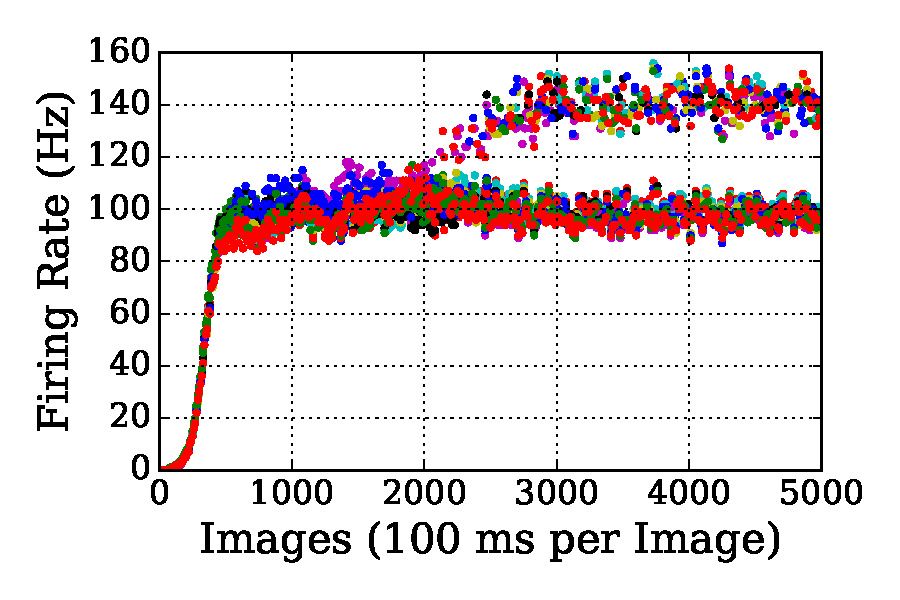
\includegraphics[width=\textwidth]{pics_sdlm/10_exp_SRBM_Orig/exp1_recon_s.pdf}
		\caption{Reconstruction of visible units in Exp1}
	\end{subfigure}
	\begin{subfigure}[t]{0.4\textwidth}
		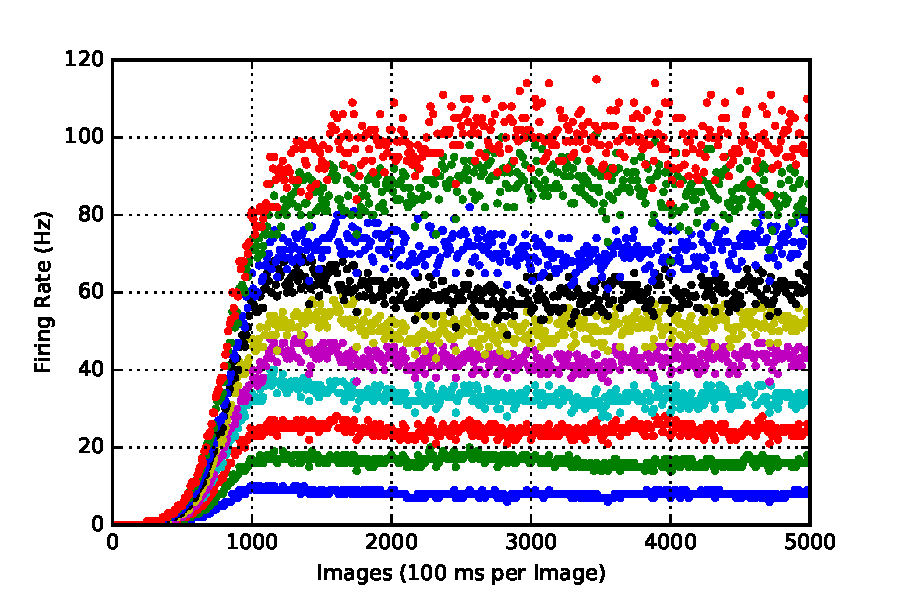
\includegraphics[width=\textwidth]{pics_sdlm/10_exp_SRBM_Orig/exp2_recon_s.pdf}
		\caption{Reconstruction of visible units in Exp2}
	\end{subfigure}\\
	\begin{subfigure}[t]{0.4\textwidth}
		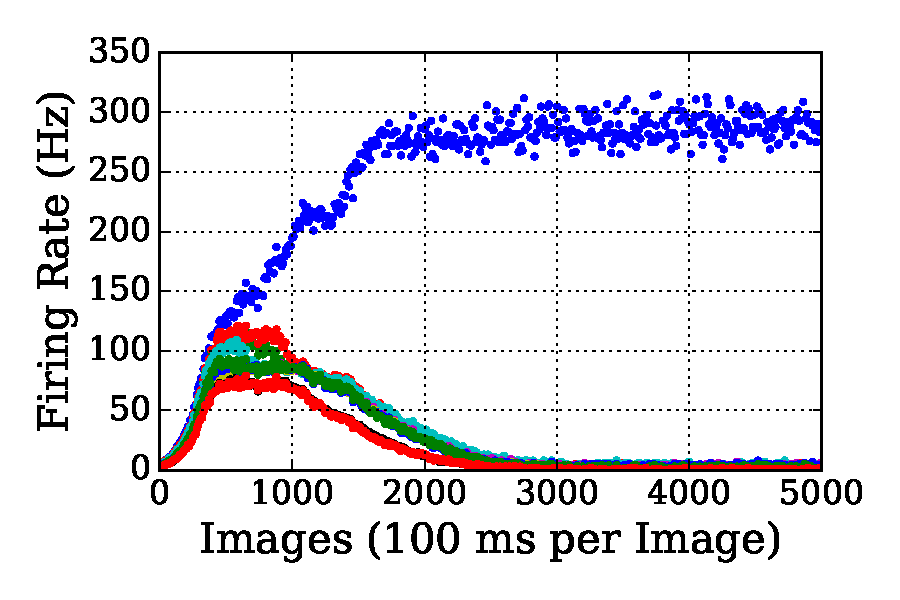
\includegraphics[width=\textwidth]{pics_sdlm/10_exp_SRBM_Orig/exp1_hid_s.pdf}
		\caption{Output of hidden units in Exp1}
	\end{subfigure}
	\begin{subfigure}[t]{0.4\textwidth}
		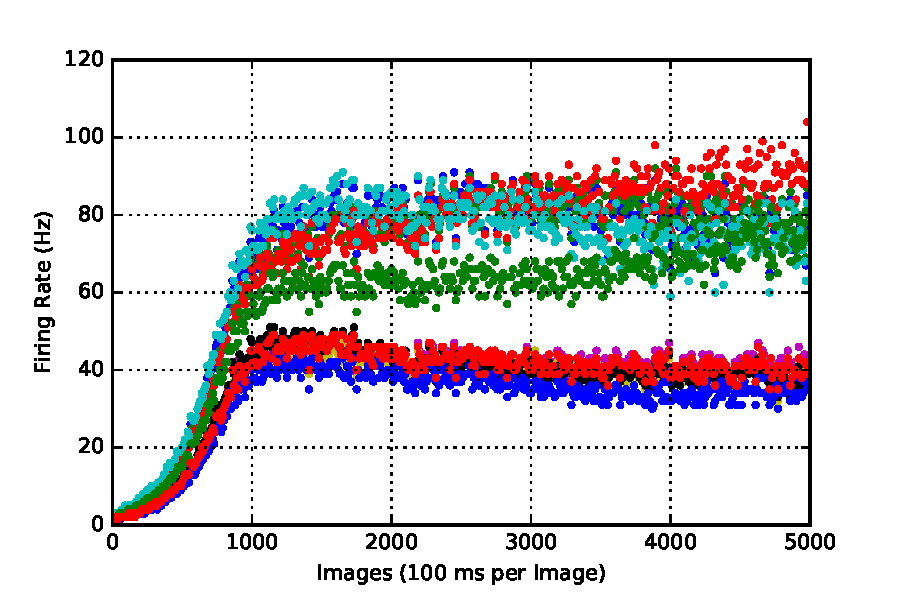
\includegraphics[width=\textwidth]{pics_sdlm/10_exp_SRBM_Orig/exp2_hid_s.pdf}
		\caption{Output of hidden units in Exp2}
	\end{subfigure}\\
	\begin{subfigure}[t]{0.4\textwidth}
		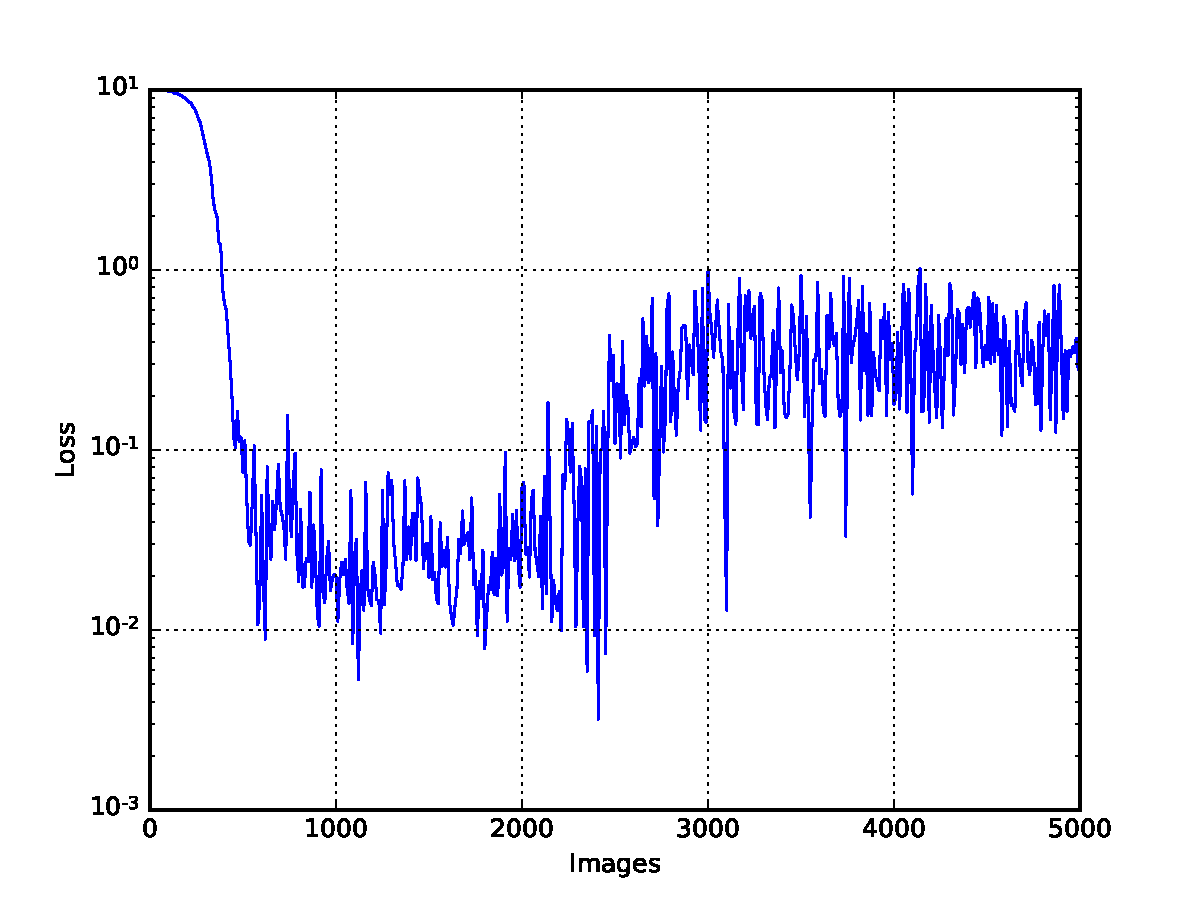
\includegraphics[width=\textwidth]{pics_sdlm/10_exp_SRBM_Orig/exp1_mse_nons.pdf}
		\caption{Loss of Exp1}
	\end{subfigure}
	\begin{subfigure}[t]{0.4\textwidth}
		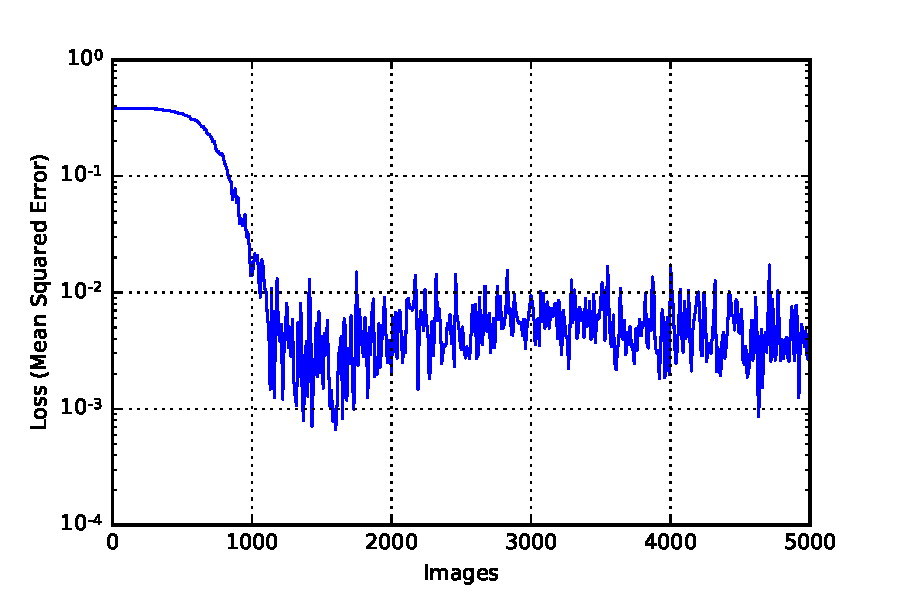
\includegraphics[width=\textwidth]{pics_sdlm/10_exp_SRBM_Orig/exp2_mse_nons.pdf}
		\caption{Loss of Exp2}
	\end{subfigure}
	\caption{Weights and firing rates of visible and hidden units change during training of the reconstruction tests of spiking RBM. 
		Experiments 1) 10 visible units fully connected to 10 hidden units with Poisson spike trains of 100~Hz which lasted 100~ms; 2) same network fed with 10 Poisson spike trains of firing rate ranging from 10~Hz to 100~Hz.}
\end{figure}

\subsection{Solution 1: Longer STDP Window}
The stronger correlation of a pair of pre- and post-synaptic neurons make the spikes generated by the post-synaptic neuron lie in the shorter period after the pre-synaptic spike.
So a longer square STDP window maker the overall weight change more dependent of the correlation of the spike trains.
\begin{figure}
	\centering
	\begin{subfigure}[t]{0.4\textwidth}
		\includegraphics[width=\textwidth]{pics_sdlm/01_exp_SAE_Orig_long/exp1_weights_s.pdf}
		\caption{Weights of Exp1}
	\end{subfigure}
	\begin{subfigure}[t]{0.4\textwidth}
		\includegraphics[width=\textwidth]{pics_sdlm/01_exp_SAE_Orig_long/exp2_weights_s.pdf}
		\caption{Weights of Exp2}
	\end{subfigure}
	\begin{subfigure}[t]{0.4\textwidth}
		\includegraphics[width=\textwidth]{pics_sdlm/01_exp_SAE_Orig_long/exp1_recon_s.pdf}
		\caption{Reconstruction of visible units in Exp1}
	\end{subfigure}
	\begin{subfigure}[t]{0.4\textwidth}
		\includegraphics[width=\textwidth]{pics_sdlm/01_exp_SAE_Orig_long/exp2_recon_s.pdf}
		\caption{Reconstruction of visible units in Exp2}
	\end{subfigure}\\
	\begin{subfigure}[t]{0.4\textwidth}
		\includegraphics[width=\textwidth]{pics_sdlm/01_exp_SAE_Orig_long/exp1_hid_s.pdf}
		\caption{Output of hidden units in Exp1}
	\end{subfigure}
	\begin{subfigure}[t]{0.4\textwidth}
		\includegraphics[width=\textwidth]{pics_sdlm/01_exp_SAE_Orig_long/exp2_hid_s.pdf}
		\caption{Output of hidden units in Exp2}
	\end{subfigure}\\
	\begin{subfigure}[t]{0.4\textwidth}
		\includegraphics[width=\textwidth]{pics_sdlm/01_exp_SAE_Orig_long/exp1_mse_nons.pdf}
		\caption{Loss of Exp1}
	\end{subfigure}
	\begin{subfigure}[t]{0.4\textwidth}
		\includegraphics[width=\textwidth]{pics_sdlm/01_exp_SAE_Orig_long/exp2_mse_nons.pdf}
		\caption{Loss of Exp2}
	\end{subfigure}
	\caption{Weights and firing rates of visible and hidden units change during training of the reconstruction tests of spiking AE. 
		Experiments 1) 10 visible units fully connected to 10 hidden units with Poisson spike trains of 100~Hz which lasted 100~ms; 2) same network fed with 10 Poisson spike trains of firing rate ranging from 10~Hz to 100~Hz.}
\end{figure}

\begin{figure}
	\centering
	\begin{subfigure}[t]{0.4\textwidth}
		\includegraphics[width=\textwidth]{pics_sdlm/11_exp_SRBM_Orig_long/exp1_weights_s.pdf}
		\caption{Weights of Exp1}
	\end{subfigure}
	\begin{subfigure}[t]{0.4\textwidth}
		\includegraphics[width=\textwidth]{pics_sdlm/11_exp_SRBM_Orig_long/exp2_weights_s.pdf}
		\caption{Weights of Exp2}
	\end{subfigure}
	\begin{subfigure}[t]{0.4\textwidth}
		\includegraphics[width=\textwidth]{pics_sdlm/11_exp_SRBM_Orig_long/exp1_recon_s.pdf}
		\caption{Reconstruction of visible units in Exp1}
	\end{subfigure}
	\begin{subfigure}[t]{0.4\textwidth}
		\includegraphics[width=\textwidth]{pics_sdlm/11_exp_SRBM_Orig_long/exp2_recon_s.pdf}
		\caption{Reconstruction of visible units in Exp2}
	\end{subfigure}\\
	\begin{subfigure}[t]{0.4\textwidth}
		\includegraphics[width=\textwidth]{pics_sdlm/11_exp_SRBM_Orig_long/exp1_hid_s.pdf}
		\caption{Output of hidden units in Exp1}
	\end{subfigure}
	\begin{subfigure}[t]{0.4\textwidth}
		\includegraphics[width=\textwidth]{pics_sdlm/11_exp_SRBM_Orig_long/exp2_hid_s.pdf}
		\caption{Output of hidden units in Exp2}
	\end{subfigure}\\
	\begin{subfigure}[t]{0.4\textwidth}
		\includegraphics[width=\textwidth]{pics_sdlm/11_exp_SRBM_Orig_long/exp1_mse_nons.pdf}
		\caption{Loss of Exp1}
	\end{subfigure}
	\begin{subfigure}[t]{0.4\textwidth}
		\includegraphics[width=\textwidth]{pics_sdlm/11_exp_SRBM_Orig_long/exp2_mse_nons.pdf}
		\caption{Loss of Exp2}
	\end{subfigure}
	\caption{Weights and firing rates of visible and hidden units change during training of the reconstruction tests of spiking RBM. 
		Experiments 1) 10 visible units fully connected to 10 hidden units with Poisson spike trains of 100~Hz which lasted 100~ms; 2) same network fed with 10 Poisson spike trains of firing rate ranging from 10~Hz to 100~Hz.}
\end{figure}
\subsection{Solution 2: Noisy Threshold}
There are various ways to introduce noise in formal spiking neuron models. In this section we focus on a `noisy threshold' (also called escape or hazard model)~\cite{gerstner2002spiking}.
The noise drives the post-synaptic spikes fire in advance or behind the expected time, thus it reduces the correlation between the pre- and post synaptic spikes.

\begin{figure}
	\centering
	\begin{subfigure}[t]{0.4\textwidth}
		\includegraphics[width=\textwidth]{pics_sdlm/03_exp_SAE_noise_long/exp1_weights_s.pdf}
		\caption{Weights of Exp1}
	\end{subfigure}
	\begin{subfigure}[t]{0.4\textwidth}
		\includegraphics[width=\textwidth]{pics_sdlm/03_exp_SAE_noise_long/exp2_weights_s.pdf}
		\caption{Weights of Exp2}
	\end{subfigure}
	\begin{subfigure}[t]{0.4\textwidth}
		\includegraphics[width=\textwidth]{pics_sdlm/03_exp_SAE_noise_long/exp1_recon_s.pdf}
		\caption{Reconstruction of visible units in Exp1}
	\end{subfigure}
	\begin{subfigure}[t]{0.4\textwidth}
		\includegraphics[width=\textwidth]{pics_sdlm/03_exp_SAE_noise_long/exp2_recon_s.pdf}
		\caption{Reconstruction of visible units in Exp2}
	\end{subfigure}\\
	\begin{subfigure}[t]{0.4\textwidth}
		\includegraphics[width=\textwidth]{pics_sdlm/03_exp_SAE_noise_long/exp1_hid_s.pdf}
		\caption{Output of hidden units in Exp1}
	\end{subfigure}
	\begin{subfigure}[t]{0.4\textwidth}
		\includegraphics[width=\textwidth]{pics_sdlm/03_exp_SAE_noise_long/exp2_hid_s.pdf}
		\caption{Output of hidden units in Exp2}
	\end{subfigure}\\
	\begin{subfigure}[t]{0.4\textwidth}
		\includegraphics[width=\textwidth]{pics_sdlm/03_exp_SAE_noise_long/exp1_mse_nons.pdf}
		\caption{Loss of Exp1}
	\end{subfigure}
	\begin{subfigure}[t]{0.4\textwidth}
		\includegraphics[width=\textwidth]{pics_sdlm/03_exp_SAE_noise_long/exp2_mse_nons.pdf}
		\caption{Loss of Exp2}
	\end{subfigure}
	\caption{Weights and firing rates of visible and hidden units change during training of the reconstruction tests of spiking AE. 
		Experiments 1) 10 visible units fully connected to 10 hidden units with Poisson spike trains of 100~Hz which lasted 100~ms; 2) same network fed with 10 Poisson spike trains of firing rate ranging from 10~Hz to 100~Hz.}
\end{figure}

\begin{figure}
	\centering
	\begin{subfigure}[t]{0.4\textwidth}
		\includegraphics[width=\textwidth]{pics_sdlm/13_exp_SRBM_noise_long/exp1_weights_s.pdf}
		\caption{Weights of Exp1}
	\end{subfigure}
	\begin{subfigure}[t]{0.4\textwidth}
		\includegraphics[width=\textwidth]{pics_sdlm/13_exp_SRBM_noise_long/exp2_weights_s.pdf}
		\caption{Weights of Exp2}
	\end{subfigure}
	\begin{subfigure}[t]{0.4\textwidth}
		\includegraphics[width=\textwidth]{pics_sdlm/13_exp_SRBM_noise_long/exp1_recon_s.pdf}
		\caption{Reconstruction of visible units in Exp1}
	\end{subfigure}
	\begin{subfigure}[t]{0.4\textwidth}
		\includegraphics[width=\textwidth]{pics_sdlm/13_exp_SRBM_noise_long/exp2_recon_s.pdf}
		\caption{Reconstruction of visible units in Exp2}
	\end{subfigure}\\
	\begin{subfigure}[t]{0.4\textwidth}
		\includegraphics[width=\textwidth]{pics_sdlm/13_exp_SRBM_noise_long/exp1_hid_s.pdf}
		\caption{Output of hidden units in Exp1}
	\end{subfigure}
	\begin{subfigure}[t]{0.4\textwidth}
		\includegraphics[width=\textwidth]{pics_sdlm/13_exp_SRBM_noise_long/exp2_hid_s.pdf}
		\caption{Output of hidden units in Exp2}
	\end{subfigure}\\
	\begin{subfigure}[t]{0.4\textwidth}
		\includegraphics[width=\textwidth]{pics_sdlm/13_exp_SRBM_noise_long/exp1_mse_nons.pdf}
		\caption{Loss of Exp1}
	\end{subfigure}
	\begin{subfigure}[t]{0.4\textwidth}
		\includegraphics[width=\textwidth]{pics_sdlm/13_exp_SRBM_noise_long/exp2_mse_nons.pdf}
		\caption{Loss of Exp2}
	\end{subfigure}
	\caption{Weights and firing rates of visible and hidden units change during training of the reconstruction tests of spiking RBM. 
		Experiments 1) 10 visible units fully connected to 10 hidden units with Poisson spike trains of 100~Hz which lasted 100~ms; 2) same network fed with 10 Poisson spike trains of firing rate ranging from 10~Hz to 100~Hz.}
\end{figure}


\subsection{Solution 3: Teaching Signal}
Teaching spike train firing at the same rate with input spikes is completely decorrelated with the spikes generated in the network.
Thus it decorrelates the positive part of the weight change (red bar in Figure~\ref{fig:rSTDP} and~\ref{fig:rSTDP_rbm}).
\begin{figure}
	\centering
	\begin{subfigure}[t]{0.4\textwidth}
		\includegraphics[width=\textwidth]{pics_sdlm/05_exp_SAE_teach_long/exp1_weights_s.pdf}
		\caption{Weights of Exp1}
	\end{subfigure}
	\begin{subfigure}[t]{0.4\textwidth}
		\includegraphics[width=\textwidth]{pics_sdlm/05_exp_SAE_teach_long/exp2_weights_s.pdf}
		\caption{Weights of Exp2}
	\end{subfigure}
	\begin{subfigure}[t]{0.4\textwidth}
		\includegraphics[width=\textwidth]{pics_sdlm/05_exp_SAE_teach_long/exp1_recon_s.pdf}
		\caption{Reconstruction of visible units in Exp1}
	\end{subfigure}
	\begin{subfigure}[t]{0.4\textwidth}
		\includegraphics[width=\textwidth]{pics_sdlm/05_exp_SAE_teach_long/exp2_recon_s.pdf}
		\caption{Reconstruction of visible units in Exp2}
	\end{subfigure}\\
	\begin{subfigure}[t]{0.4\textwidth}
		\includegraphics[width=\textwidth]{pics_sdlm/05_exp_SAE_teach_long/exp1_hid_s.pdf}
		\caption{Output of hidden units in Exp1}
	\end{subfigure}
	\begin{subfigure}[t]{0.4\textwidth}
		\includegraphics[width=\textwidth]{pics_sdlm/05_exp_SAE_teach_long/exp2_hid_s.pdf}
		\caption{Output of hidden units in Exp2}
	\end{subfigure}\\
	\begin{subfigure}[t]{0.4\textwidth}
		\includegraphics[width=\textwidth]{pics_sdlm/05_exp_SAE_teach_long/exp1_mse_nons.pdf}
		\caption{Loss of Exp1}
	\end{subfigure}
	\begin{subfigure}[t]{0.4\textwidth}
		\includegraphics[width=\textwidth]{pics_sdlm/05_exp_SAE_teach_long/exp2_mse_nons.pdf}
		\caption{Loss of Exp2}
	\end{subfigure}
	\caption{Weights and firing rates of visible and hidden units change during training of the reconstruction tests of spiking AE. 
		Experiments 1) 10 visible units fully connected to 10 hidden units with Poisson spike trains of 100~Hz which lasted 100~ms; 2) same network fed with 10 Poisson spike trains of firing rate ranging from 10~Hz to 100~Hz.}
\end{figure}

\begin{figure}
	\centering
	\begin{subfigure}[t]{0.4\textwidth}
		\includegraphics[width=\textwidth]{pics_sdlm/15_exp_SRBM_teach_long/exp1_weights_s.pdf}
		\caption{Weights of Exp1}
	\end{subfigure}
	\begin{subfigure}[t]{0.4\textwidth}
		\includegraphics[width=\textwidth]{pics_sdlm/15_exp_SRBM_teach_long/exp2_weights_s.pdf}
		\caption{Weights of Exp2}
	\end{subfigure}
	\begin{subfigure}[t]{0.4\textwidth}
		\includegraphics[width=\textwidth]{pics_sdlm/15_exp_SRBM_teach_long/exp1_recon_s.pdf}
		\caption{Reconstruction of visible units in Exp1}
	\end{subfigure}
	\begin{subfigure}[t]{0.4\textwidth}
		\includegraphics[width=\textwidth]{pics_sdlm/15_exp_SRBM_teach_long/exp2_recon_s.pdf}
		\caption{Reconstruction of visible units in Exp2}
	\end{subfigure}\\
	\begin{subfigure}[t]{0.4\textwidth}
		\includegraphics[width=\textwidth]{pics_sdlm/15_exp_SRBM_teach_long/exp1_hid_s.pdf}
		\caption{Output of hidden units in Exp1}
	\end{subfigure}
	\begin{subfigure}[t]{0.4\textwidth}
		\includegraphics[width=\textwidth]{pics_sdlm/15_exp_SRBM_teach_long/exp2_hid_s.pdf}
		\caption{Output of hidden units in Exp2}
	\end{subfigure}\\
	\begin{subfigure}[t]{0.4\textwidth}
		\includegraphics[width=\textwidth]{pics_sdlm/15_exp_SRBM_teach_long/exp1_mse_nons.pdf}
		\caption{Loss of Exp1}
	\end{subfigure}
	\begin{subfigure}[t]{0.4\textwidth}
		\includegraphics[width=\textwidth]{pics_sdlm/15_exp_SRBM_teach_long/exp2_mse_nons.pdf}
		\caption{Loss of Exp2}
	\end{subfigure}
	\caption{Weights and firing rates of visible and hidden units change during training of the reconstruction tests of spiking RBM. 
		Experiments 1) 10 visible units fully connected to 10 hidden units with Poisson spike trains of 100~Hz which lasted 100~ms; 2) same network fed with 10 Poisson spike trains of firing rate ranging from 10~Hz to 100~Hz.}
\end{figure}

\subsection{Test on Combined Solutions}
Same test:
\begin{figure}
	\centering
	\begin{subfigure}[t]{0.4\textwidth}
		\includegraphics[width=\textwidth]{pics_sdlm/07_exp_SAE_all_long/exp1_weights_s.pdf}
		\caption{Weights of Exp1}
	\end{subfigure}
	\begin{subfigure}[t]{0.4\textwidth}
		\includegraphics[width=\textwidth]{pics_sdlm/07_exp_SAE_all_long/exp2_weights_s.pdf}
		\caption{Weights of Exp2}
	\end{subfigure}
	\begin{subfigure}[t]{0.4\textwidth}
		\includegraphics[width=\textwidth]{pics_sdlm/07_exp_SAE_all_long/exp1_recon_s.pdf}
		\caption{Reconstruction of visible units in Exp1}
	\end{subfigure}
	\begin{subfigure}[t]{0.4\textwidth}
		\includegraphics[width=\textwidth]{pics_sdlm/07_exp_SAE_all_long/exp2_recon_s.pdf}
		\caption{Reconstruction of visible units in Exp2}
	\end{subfigure}\\
	\begin{subfigure}[t]{0.4\textwidth}
		\includegraphics[width=\textwidth]{pics_sdlm/07_exp_SAE_all_long/exp1_hid_s.pdf}
		\caption{Output of hidden units in Exp1}
	\end{subfigure}
	\begin{subfigure}[t]{0.4\textwidth}
		\includegraphics[width=\textwidth]{pics_sdlm/07_exp_SAE_all_long/exp2_hid_s.pdf}
		\caption{Output of hidden units in Exp2}
	\end{subfigure}\\
	\begin{subfigure}[t]{0.4\textwidth}
		\includegraphics[width=\textwidth]{pics_sdlm/07_exp_SAE_all_long/exp1_mse_nons.pdf}
		\caption{Loss of Exp1}
	\end{subfigure}
	\begin{subfigure}[t]{0.4\textwidth}
		\includegraphics[width=\textwidth]{pics_sdlm/07_exp_SAE_all_long/exp2_mse_nons.pdf}
		\caption{Loss of Exp2}
	\end{subfigure}
	\caption{Weights and firing rates of visible and hidden units change during training of the reconstruction tests of spiking AE. 
		Experiments 1) 10 visible units fully connected to 10 hidden units with Poisson spike trains of 100~Hz which lasted 100~ms; 2) same network fed with 10 Poisson spike trains of firing rate ranging from 10~Hz to 100~Hz.}
\end{figure}

\begin{figure}
	\centering
	\begin{subfigure}[t]{0.4\textwidth}
		\includegraphics[width=\textwidth]{pics_sdlm/17_exp_SRBM_all_long/exp1_weights_s.pdf}
		\caption{Weights of Exp1}
	\end{subfigure}
	\begin{subfigure}[t]{0.4\textwidth}
		\includegraphics[width=\textwidth]{pics_sdlm/17_exp_SRBM_all_long/exp2_weights_s.pdf}
		\caption{Weights of Exp2}
	\end{subfigure}
	\begin{subfigure}[t]{0.4\textwidth}
		\includegraphics[width=\textwidth]{pics_sdlm/17_exp_SRBM_all_long/exp1_recon_s.pdf}
		\caption{Reconstruction of visible units in Exp1}
	\end{subfigure}
	\begin{subfigure}[t]{0.4\textwidth}
		\includegraphics[width=\textwidth]{pics_sdlm/17_exp_SRBM_all_long/exp2_recon_s.pdf}
		\caption{Reconstruction of visible units in Exp2}
	\end{subfigure}\\
	\begin{subfigure}[t]{0.4\textwidth}
		\includegraphics[width=\textwidth]{pics_sdlm/17_exp_SRBM_all_long/exp1_hid_s.pdf}
		\caption{Output of hidden units in Exp1}
	\end{subfigure}
	\begin{subfigure}[t]{0.4\textwidth}
		\includegraphics[width=\textwidth]{pics_sdlm/17_exp_SRBM_all_long/exp2_hid_s.pdf}
		\caption{Output of hidden units in Exp2}
	\end{subfigure}\\
	\begin{subfigure}[t]{0.4\textwidth}
		\includegraphics[width=\textwidth]{pics_sdlm/17_exp_SRBM_all_long/exp1_mse_nons.pdf}
		\caption{Loss of Exp1}
	\end{subfigure}
	\begin{subfigure}[t]{0.4\textwidth}
		\includegraphics[width=\textwidth]{pics_sdlm/17_exp_SRBM_all_long/exp2_mse_nons.pdf}
		\caption{Loss of Exp2}
	\end{subfigure}
	\caption{Weights and firing rates of visible and hidden units change during training of the reconstruction tests of spiking RBM. 
		Experiments 1) 10 visible units fully connected to 10 hidden units with Poisson spike trains of 100~Hz which lasted 100~ms; 2) same network fed with 10 Poisson spike trains of firing rate ranging from 10~Hz to 100~Hz.}
\end{figure}

XOR problem:
To validate the decorrelation methods proposed, a more complicated reconstruction experiment is conducted.
The input nodes are fed with values (x, y, z) sequentially (0, 0, 0), (0, 1, 1), (1, 0, 1) and (1, 1, 0) which follows XOR rules, z = x XOR y.
9 visible units presented values of (x, y, z) by group of 3 and were fed with values of (0, 0, 0), (0, 1, 1), (1, 0, 1), (1, 1, 0) repeatedly with 100~ms Poisson spike trains firing at 100~Hz for 1, 0~Hz otherwise. And the visible units were fully connected to 9 hidden units.
\begin{figure}
	\centering
	\begin{subfigure}[t]{0.32\textwidth}
		\includegraphics[width=\textwidth]{pics_sdlm/21_exp_AE_noise/exp3_weights_s.pdf}
		\caption{Weights of AE}
	\end{subfigure}
	\begin{subfigure}[t]{0.32\textwidth}
		\includegraphics[width=\textwidth]{pics_sdlm/00_exp_SAE_Orig/exp3_weights_s.pdf}
		\caption{Weights of Original SAE}
	\end{subfigure}
	\begin{subfigure}[t]{0.32\textwidth}
		\includegraphics[width=\textwidth]{pics_sdlm/07_exp_SAE_all_long/exp3_weights_s.pdf}
		\caption{Weights of Optimised SAE}
	\end{subfigure}\\
	\begin{subfigure}[t]{0.32\textwidth}
		\includegraphics[width=\textwidth]{pics_sdlm/21_exp_AE_noise/exp3_recon_s2.pdf}
		\caption{Reconstruction of visible units in AE}
	\end{subfigure}
	\begin{subfigure}[t]{0.32\textwidth}
		\includegraphics[width=\textwidth]{pics_sdlm/00_exp_SAE_Orig/exp3_recon_s_2.pdf}
		\caption{Reconstruction of visible units in Original SAE}
	\end{subfigure}
	\begin{subfigure}[t]{0.32\textwidth}
		\includegraphics[width=\textwidth]{pics_sdlm/07_exp_SAE_all_long/exp3_recon_s_2.pdf}
		\caption{Reconstruction of visible units in Optimised SAE}
	\end{subfigure}\\
	\begin{subfigure}[t]{0.32\textwidth}
		\includegraphics[width=\textwidth]{pics_sdlm/21_exp_AE_noise/exp3_hid_s_2.pdf}
		\caption{Output of hidden units in AE}
	\end{subfigure}
	\begin{subfigure}[t]{0.32\textwidth}
		\includegraphics[width=\textwidth]{pics_sdlm/00_exp_SAE_Orig/exp3_hid_s_2.pdf}
		\caption{Output of hidden units in Original SAE}
	\end{subfigure}
	\begin{subfigure}[t]{0.32\textwidth}
		\includegraphics[width=\textwidth]{pics_sdlm/07_exp_SAE_all_long/exp3_hid_s_2.pdf}
		\caption{Output of hidden units in Optimised SAE}
	\end{subfigure}\\
	\begin{subfigure}[t]{0.32\textwidth}
		\includegraphics[width=\textwidth]{pics_sdlm/21_exp_AE_noise/exp3_loss_s_2.pdf}
		\caption{Loss of AE}
	\end{subfigure}
	\begin{subfigure}[t]{0.32\textwidth}
		\includegraphics[width=\textwidth]{pics_sdlm/00_exp_SAE_Orig/exp3_mse_nons_2.pdf}
		\caption{Loss of Original SAE}
	\end{subfigure}
	\begin{subfigure}[t]{0.32\textwidth}
		\includegraphics[width=\textwidth]{pics_sdlm/07_exp_SAE_all_long/exp3_mse_nons_2.pdf}
		\caption{Loss of Optimised SAE}
	\end{subfigure}
	\caption{Experiment 3) Weights and firing rates of visible and hidden units change during training of the reconstruction tests of AE and spiking AE.}
\end{figure}

\begin{figure}
	\centering
	\begin{subfigure}[t]{0.32\textwidth}
		\includegraphics[width=\textwidth]{pics_sdlm/31_exp_RBM_noise/exp3_weights_s.pdf}
		\caption{Weights of RBM}
	\end{subfigure}
	\begin{subfigure}[t]{0.32\textwidth}
		\includegraphics[width=\textwidth]{pics_sdlm/10_exp_SRBM_Orig/exp3_weights_s.pdf}
		\caption{Weights of Original SRBM}
	\end{subfigure}
	\begin{subfigure}[t]{0.32\textwidth}
		\includegraphics[width=\textwidth]{pics_sdlm/17_exp_SRBM_all_long/exp3_weights_s.pdf}
		\caption{Weights of Optimised SRBM}
	\end{subfigure}\\
	\begin{subfigure}[t]{0.32\textwidth}
		\includegraphics[width=\textwidth]{pics_sdlm/31_exp_RBM_noise/exp3_recon_s2.pdf}
		\caption{Reconstruction of visible units in RBM}
	\end{subfigure}
	\begin{subfigure}[t]{0.32\textwidth}
		\includegraphics[width=\textwidth]{pics_sdlm/10_exp_SRBM_Orig/exp3_recon_s_2.pdf}
		\caption{Reconstruction of visible units in Original SRBM}
	\end{subfigure}
	\begin{subfigure}[t]{0.32\textwidth}
		\includegraphics[width=\textwidth]{pics_sdlm/17_exp_SRBM_all_long/exp3_recon_s_2.pdf}
		\caption{Reconstruction of visible units in Optimised SRBM}
	\end{subfigure}\\
	\begin{subfigure}[t]{0.32\textwidth}
		\includegraphics[width=\textwidth]{pics_sdlm/31_exp_RBM_noise/exp3_hid_s_2.pdf}
		\caption{Output of hidden units in RBM}
	\end{subfigure}
	\begin{subfigure}[t]{0.32\textwidth}
		\includegraphics[width=\textwidth]{pics_sdlm/10_exp_SRBM_Orig/exp3_hid_s_2.pdf}
		\caption{Output of hidden units in Original SRBM}
	\end{subfigure}
	\begin{subfigure}[t]{0.32\textwidth}
		\includegraphics[width=\textwidth]{pics_sdlm/17_exp_SRBM_all_long/exp3_hid_s_2.pdf}
		\caption{Output of hidden units in Optimised SRBM}
	\end{subfigure}\\
	\begin{subfigure}[t]{0.32\textwidth}
		\includegraphics[width=\textwidth]{pics_sdlm/31_exp_RBM_noise/exp3_loss_s_2.pdf}
		\caption{Loss of Optimised RBM}
	\end{subfigure}
	\begin{subfigure}[t]{0.32\textwidth}
		\includegraphics[width=\textwidth]{pics_sdlm/10_exp_SRBM_Orig/exp3_mse_nons_2.pdf}
		\caption{Loss of Original SRBM}
	\end{subfigure}
	\begin{subfigure}[t]{0.32\textwidth}
		\includegraphics[width=\textwidth]{pics_sdlm/17_exp_SRBM_all_long/exp3_mse_nons_2.pdf}
		\caption{Loss of Optimised SRBM}
	\end{subfigure}
	\caption{Experiment 3) Weights and firing rates of visible and hidden units change during training of the reconstruction tests of RBM and spiking SRBM.}
\end{figure}


\section{Results: MNIST Test}
MNIST structure.
As the baseline to compare with, the same neural network architecture was firstly tested on original AE and nRBM, and then trained on SNNs.
Three epochs of all the $60,000$ training images were fed into the network in order.
In the training of SNNs, pixel values of images were represented by spike trains firing at certain frequency linear to the original value.
Therefore the over all count of spikes for each pixel is equivalent to adding Gaussian noise to its value.
To provide an equal comparison, the pixel values counted by the same spike trains used in SNNs were also applied to the original ANN training.
\begin{figure}
	\centering
	\includegraphics[width=0.6\textwidth]{pics_sdlm/mnist.pdf}
	\caption{AE and RBM structure for MNIST tasks.}
	\label{fig:MNSIT}
\end{figure}
\subsection{Trained weights}
AE automatically extracts features.

\begin{figure}
	\centering
	\begin{subfigure}[t]{0.4\textwidth}
		\includegraphics[width=\textwidth]{pics_sdlm/22_MNIST_AE/2_60000_0.pdf}
		\caption{AE}
	\end{subfigure}
	\begin{subfigure}[t]{0.4\textwidth}
		\includegraphics[width=\textwidth]{pics_sdlm/23_MNIST_AE_noise/2_60000_0.pdf}
		\caption{AE+Poisson input}
	\end{subfigure}\\
	\begin{subfigure}[t]{0.4\textwidth}
		\includegraphics[width=\textwidth]{pics_sdlm/40_MNIST_SAE_original/2_60000_0.pdf}
		\caption{SAE}
	\end{subfigure}
	\begin{subfigure}[t]{0.4\textwidth}
		\includegraphics[width=\textwidth]{pics_sdlm/41_MNIST_SAE_teach/2_60000_0.pdf}
		\caption{SAE+teaching signal.}
	\end{subfigure}\\
	\begin{subfigure}[t]{0.4\textwidth}
		\includegraphics[width=\textwidth]{pics_sdlm/noise_ae/2_60000_0.pdf}
		\caption{SAE+noisy threshold.}
	\end{subfigure}
	\begin{subfigure}[t]{0.4\textwidth}
		\includegraphics[width=\textwidth]{pics_sdlm/43_MNIST_SAE_all/2_60000_0.pdf}
		\caption{SAE+teach+noise.}
	\end{subfigure}\\
	\caption{Trained weights after training 3 epochs of MNIST data using (a) AE, (b) AE with Poisson spike trains as input data, (c) Original SAE, (d) SAE trained with extra teaching signal, (e) SAE trained with neurons of noisy threshold, and (f) SAE trained with both solutions.}
\end{figure}

\begin{figure}
	\centering
	\begin{subfigure}[t]{0.4\textwidth}
		\includegraphics[width=\textwidth]{pics_sdlm/32_MNIST_RBM/2_60000_0.pdf}
		\caption{nRBM}
	\end{subfigure}
	\begin{subfigure}[t]{0.4\textwidth}
		\includegraphics[width=\textwidth]{pics_sdlm/33_MNIST_RBM_noise/2_60000_0.pdf}
		\caption{nRBM+Poisson input}
	\end{subfigure}\\
	\begin{subfigure}[t]{0.4\textwidth}
		\includegraphics[width=\textwidth]{pics_sdlm/50_MNIST_SRBM_original/2_60000_0.pdf}
		\caption{SRBM}
	\end{subfigure}
	\begin{subfigure}[t]{0.4\textwidth}
		\includegraphics[width=\textwidth]{pics_sdlm/51_MNIST_SRBM_teach/2_60000_0.pdf}
		\caption{SRBM+teaching signal.}
	\end{subfigure}\\
	\begin{subfigure}[t]{0.4\textwidth}
		\includegraphics[width=\textwidth]{pics_sdlm/noise_rbm/2_60000_0.pdf}
		\caption{SRBM+noisy threshold.}
	\end{subfigure}
	\begin{subfigure}[t]{0.4\textwidth}
		\includegraphics[width=\textwidth]{pics_sdlm/53_MNIST_SRBM_all/2_60000_0.pdf}
		\caption{SRBM+teach+noise.}
	\end{subfigure}\\
	\caption{Trained weights after training 3 epochs of MNIST data using (a) nRBM, (b) nRBM with Poisson spike trains as input data, (c) Original SRBM, (d) SRBM trained with extra teaching signal, (e) SRBM trained with neurons of noisy threshold, and (f) SRBM trained with both solutions.}
\end{figure}

\subsection{Classification Accuracy}
Original AE and nRBM.
%\begin{figure}
%	\centering
%	\includegraphics[width=0.6\textwidth]{pics_sdlm/33_MNIST_RBM_noise/non_spike_MNIST.pdf}
%	\caption{Classification accuracy tested on original AE and nRBM.}
%	\label{fig:non_mnist_result}
%\end{figure}

\begin{figure}
	\centering
	\begin{subfigure}[t]{0.45\textwidth}
		\includegraphics[width=\textwidth]{pics_sdlm/43_MNIST_SAE_all/compare_result.pdf}
		\caption{Classification accuracy compared on AE and SAEs.}
	\end{subfigure}
	\begin{subfigure}[t]{0.45\textwidth}
		\includegraphics[width=\textwidth]{pics_sdlm/53_MNIST_SRBM_all/compare_result.pdf}
		\caption{Classification accuracy compared on RBM and SRBMs.}
	\end{subfigure}
	\caption{Classification Accuracy compared with traditional training method and spike-based STDP learning.}
\end{figure}

\subsection{Reconstruction}
AE reconstructs visible units.
\begin{figure}
	\centering
	\begin{subfigure}[t]{0.45\textwidth}
		\includegraphics[width=\textwidth]{pics_sdlm/53_MNIST_SRBM_all/compare_recon.pdf}
		\caption{Loss compared on AE and SAEs.}
	\end{subfigure}
	\begin{subfigure}[t]{0.45\textwidth}
		\includegraphics[width=\textwidth]{pics_sdlm/53_MNIST_SRBM_all/compare_recon_rbm.pdf}
		\caption{Loss compared on RBM and SRBMs.}
	\end{subfigure}
	\caption{Loss (mean squared error) compared with traditional training method and spike-based STDP learning.}
\end{figure}


\begin{figure}
	\centering
	\begin{subfigure}[t]{0.32\textwidth}
		\includegraphics[width=\textwidth]{pics_sdlm/22_MNIST_AE/recon_digit.pdf}
		\caption{AE}
	\end{subfigure}
	\begin{subfigure}[t]{0.32\textwidth}
		\includegraphics[width=\textwidth]{pics_sdlm/23_MNIST_AE_noise/recon_digit.pdf}
		\caption{AE+Poisson input}
	\end{subfigure}
	\begin{subfigure}[t]{0.32\textwidth}
		\includegraphics[width=\textwidth]{pics_sdlm/40_MNIST_SAE_original/recon_digit.pdf}
		\caption{SAE}
	\end{subfigure}\\
	\begin{subfigure}[t]{0.32\textwidth}
		\includegraphics[width=\textwidth]{pics_sdlm/41_MNIST_SAE_teach/recon_digit.pdf}
		\caption{SAE+teaching signal.}
	\end{subfigure}
	\begin{subfigure}[t]{0.32\textwidth}
		\includegraphics[width=\textwidth]{pics_sdlm/noise_ae/recon_digit.pdf}
		\caption{SAE+noisy threshold.}
	\end{subfigure}
	\begin{subfigure}[t]{0.32\textwidth}
		\includegraphics[width=\textwidth]{pics_sdlm/43_MNIST_SAE_all/recon_digit.pdf}
		\caption{SAE+teach+noise.}
	\end{subfigure}\\
	\caption{Reconstruct of the same digit '2' with trained weights using (a) AE, (b) AE with Poisson spike trains as input data, (c) Original SAE, (d) SAE trained with extra teaching signal, (e) SAE trained with neurons of noisy threshold, and (f) SAE trained with both solutions.}
\end{figure}

\begin{figure}
	\centering
	\begin{subfigure}[t]{0.32\textwidth}
		\includegraphics[width=\textwidth]{pics_sdlm/32_MNIST_RBM/recon_digit.pdf}
		\caption{nRBM}
	\end{subfigure}
	\begin{subfigure}[t]{0.32\textwidth}
		\includegraphics[width=\textwidth]{pics_sdlm/33_MNIST_RBM_noise/recon_digit.pdf}
		\caption{nRBM+Poisson input}
	\end{subfigure}
	\begin{subfigure}[t]{0.32\textwidth}
		\includegraphics[width=\textwidth]{pics_sdlm/50_MNIST_SRBM_original/recon_digit.pdf}
		\caption{SRBM}
	\end{subfigure}\\
	\begin{subfigure}[t]{0.32\textwidth}
		\includegraphics[width=\textwidth]{pics_sdlm/51_MNIST_SRBM_teach/recon_digit.pdf}
		\caption{SRBM+teaching signal.}
	\end{subfigure}
	\begin{subfigure}[t]{0.32\textwidth}
		\includegraphics[width=\textwidth]{pics_sdlm/noise_rbm/recon_digit.pdf}
		\caption{SRBM+noisy threshold.}
	\end{subfigure}
	\begin{subfigure}[t]{0.32\textwidth}
		\includegraphics[width=\textwidth]{pics_sdlm/53_MNIST_SRBM_all/recon_digit.pdf}
		\caption{SRBM+teach+noise.}
	\end{subfigure}\\
	\caption{Reconstruct of the same digit '2' with trained weights using (a) nRBM, (b) nRBM with Poisson spike trains as input data, (c) Original SRBM, (d) SRBM trained with extra teaching signal, (e) SRBM trained with neurons of noisy threshold, and (f) SRBM trained with both solutions.}
\end{figure}




\subsection{Classification Latency}
\begin{figure}
	\centering
	\begin{subfigure}[t]{0.4\textwidth}
		\includegraphics[width=\textwidth]{pics_sdlm/40_MNIST_SAE_original/latency.pdf}
		\caption{SAE}
	\end{subfigure}
	\begin{subfigure}[t]{0.4\textwidth}
		\includegraphics[width=\textwidth]{pics_sdlm/41_MNIST_SAE_teach/latency.pdf}
		\caption{SAE+teach}
	\end{subfigure}\\
	\begin{subfigure}[t]{0.4\textwidth}
		\includegraphics[width=\textwidth]{pics_sdlm/noise_ae/latency.pdf}
		\caption{SAE+noise}
	\end{subfigure}
	\begin{subfigure}[t]{0.4\textwidth}
		\includegraphics[width=\textwidth]{pics_sdlm/43_MNIST_SAE_all/latency.pdf}
		\caption{SAE+teaching signal}
	\end{subfigure}
	\caption{Classification accuracy during the entire testing time period for SAEs.}
\end{figure}

\begin{figure}
	\centering
	\begin{subfigure}[t]{0.4\textwidth}
		\includegraphics[width=\textwidth]{pics_sdlm/50_MNIST_SRBM_original/latency.pdf}
		\caption{SRBM}
	\end{subfigure}
	\begin{subfigure}[t]{0.4\textwidth}
		\includegraphics[width=\textwidth]{pics_sdlm/51_MNIST_SRBM_teach/latency.pdf}
		\caption{SRBM+teach}
	\end{subfigure}\\
	\begin{subfigure}[t]{0.4\textwidth}
		\includegraphics[width=\textwidth]{pics_sdlm/noise_rbm/latency.pdf}
		\caption{SRBM+noise.}
	\end{subfigure}
	\begin{subfigure}[t]{0.4\textwidth}
		\includegraphics[width=\textwidth]{pics_sdlm/53_MNIST_SRBM_all/latency.pdf}
		\caption{SRBM+teach+noise}
	\end{subfigure}
	\caption{Classification accuracy during the entire testing time period for SRBMs.}
\end{figure}

\subsubsection{Energy Consumption}
Latency$\times$Sops$\times$ops/s

\begin{figure}
	\centering
	\begin{subfigure}[t]{0.45\textwidth}
		\includegraphics[width=\textwidth]{pics_sdlm/43_MNIST_SAE_all/result_freq.pdf}
		\caption{SAE+teach+noise.}
	\end{subfigure}
	\begin{subfigure}[t]{0.45\textwidth}
		\includegraphics[width=\textwidth]{pics_sdlm/51_MNIST_SRBM_teach/result_freq.pdf}
		\caption{SRBM+teach+noise.}
	\end{subfigure}
	\caption{Classification accuracy during the entire testing time period with increasing input spike firing rate.}
\end{figure}

\section{Conclusion}
%A conclusion should be a short summary of the most pithy points in the chapter. It’s the thing that you’re going to leave the reader with. Given that they’ve just spent time reading the whole chapter, they don’t want to read it all again. What do you most want the reader to remember about this chapter? What is the key to the argument you’ve made, the most significant thing(s) that they have to keep in their mind as they go forward? In a thesis, a conclusion is usually fairly brief and to the point. Barbara and I call this ‘crunching’. Crunching the conclusion requires some thought – it’s not an afterthought. It is always about your take-home message, if you like. So don’t go on at length in the conclusion – Crunch.
\section{Appendices}
\subsection{Derivation process of Equation~(\ref{equ:part})}
\label{app:part}
\begin{equation}
\begin{aligned}
\dfrac{\partial \log Z(\Theta)}{\partial \theta}
=&\frac{1}{Z(\Theta)}\dfrac{\partial Z(\Theta)}{\partial \theta}\\
=&\frac{1}{Z(\Theta)} \int \dfrac{\partial f(\mathbf{x} \mid \Theta)}{\partial \theta} \D \mathbf{x} \\
=&\frac{1}{Z(\Theta)} \int f(\mathbf{x} \mid \Theta) \frac{1}{f(\mathbf{x} \mid \Theta)} \dfrac{\partial  f(\mathbf{x} \mid \Theta)}{\partial \theta} \D \mathbf{x}\\
=& \int \frac{f(\mathbf{x} \mid \Theta) }{Z(\Theta)} \dfrac{\partial \log f(\mathbf{x} \mid \Theta)}{\partial \theta} \D \mathbf{x}\\
=& \int  p(\mathbf{x} \mid \Theta) \dfrac{\partial \log f(\mathbf{x} \mid \Theta)}{\partial \theta} \D \mathbf{x}\\
=&\left \langle \dfrac{\partial \log f(\mathbf{c} \mid \Theta)}{\partial \theta}\right \rangle_{\mathbf{C} \sim p(\mathbf{x} \mid \Theta)}
\end{aligned}
\end{equation}
\subsection{Derivation process of Equation~(\ref{equ:RBM})  }
\label{app:RBM}
\begin{equation}
\begin{aligned}
\dfrac{\partial \hat{l} (\Theta \mid \mathbf{D})}{\partial \theta} 
& = \left \langle \dfrac{\partial \log f(\mathbf{d} \mid \Theta)}{\partial \theta}\right \rangle_{\mathbf{V=D}} -\left \langle \dfrac{\partial \log f(\mathbf{v} \mid \Theta)}{\partial \theta}\right \rangle_{\mathbf{V} \sim p(\mathbf{x} \mid \Theta)}  \\
& = \left \langle \dfrac{\partial \log \sum_{ \mathbf{h}} e^{-E(\mathbf{v}, \mathbf{h} \mid \Theta)}}{\partial \theta}\right \rangle_{\mathbf{V}} 
-\left \langle \dfrac{\partial \log \sum_{ \mathbf{h}} e^{-E(\mathbf{v}, \mathbf{h} \mid \Theta)} }{\partial \theta}\right \rangle_{\mathbf{V} \sim p(\mathbf{v} \mid \Theta)}  \\
& = \left \langle \sum_{ \mathbf{h}} \frac{e^{-E(\mathbf{v}, \mathbf{h} \mid \Theta)}}{\sum_{ \mathbf{h}} e^{-E(\mathbf{v}, \mathbf{h} \mid \Theta)}} \cdot \dfrac{\partial -E(\mathbf{v}, \mathbf{h} \mid \Theta)}{\partial \theta} \right \rangle_{\mathbf{V}} 
- \left \langle \sum_{ \mathbf{h}} \frac{e^{-E(\mathbf{v}, \mathbf{h} \mid \Theta)}}{\sum_{ \mathbf{h}} e^{-E(\mathbf{v}, \mathbf{h} \mid \Theta)}} \cdot \dfrac{\partial -E(\mathbf{v}, \mathbf{h} \mid \Theta)}{\partial \theta} \right \rangle_{\mathbf{V} \sim p(\mathbf{v} \mid \Theta)}  \\
& = \left \langle \sum_{ \mathbf{h}} \frac{p(\mathbf{v}, \mathbf{h} \mid \Theta)}{p(\mathbf{v} \mid \Theta)} \cdot \dfrac{\partial -E(\mathbf{v}, \mathbf{h} \mid \Theta)}{\partial \theta} \right \rangle_{\mathbf{V}} 
- \left \langle \sum_{ \mathbf{h}}  \frac{p(\mathbf{v}, \mathbf{h} \mid \Theta)}{p(\mathbf{v} \mid \Theta)} \cdot \dfrac{\partial -E(\mathbf{v}, \mathbf{h} \mid \Theta)}{\partial \theta} \right \rangle_{\mathbf{V} \sim p(\mathbf{v} \mid \Theta)}  \\
& = \left \langle \sum_{ \mathbf{h}} p( \mathbf{h} \mid \mathbf{v}, \Theta) \cdot \dfrac{\partial -E(\mathbf{v}, \mathbf{h} \mid \Theta)}{\partial \theta} \right \rangle_{\mathbf{V}} 
- \left \langle \sum_{ \mathbf{h}} p( \mathbf{h} \mid \mathbf{v}, \Theta) \cdot \dfrac{\partial -E(\mathbf{v}, \mathbf{h} \mid \Theta)}{\partial \theta} \right \rangle_{\mathbf{V} \sim p(\mathbf{v} \mid \Theta)}  \\
& = \left \langle \left \langle \dfrac{\partial -E(\mathbf{v}, \mathbf{h} \mid \Theta)}{\partial \theta} \right \rangle_{\mathbf{h} \sim p( \mathbf{h} \mid \mathbf{v}, \Theta)} \right \rangle_{\mathbf{V}}
- \left \langle \left \langle \dfrac{\partial -E(\mathbf{v}, \mathbf{h} \mid \Theta)}{\partial \theta} \right \rangle_{\mathbf{h} \sim p( \mathbf{h} \mid \mathbf{v}, \Theta)} \right \rangle_{\mathbf{V} \sim p(\mathbf{v} \mid \Theta)}  \\
& = \left \langle \dfrac{\partial -E(\mathbf{v}, \mathbf{h} \mid \Theta)}{\partial \theta} \right \rangle_{\mathbf{h} \sim p( \mathbf{h} \mid \mathbf{v}, \Theta), \mathbf{V}} 
- \left \langle \dfrac{\partial -E(\mathbf{v}, \mathbf{h} \mid \Theta)}{\partial \theta} \right \rangle_{\mathbf{v}, \mathbf{h} \sim p( \mathbf{v}, \mathbf{h} \mid  \Theta)}  \\
\end{aligned}
\end{equation}